\documentclass[oneside]{risethesis}
\usepackage{natbib}
\usepackage{babel}
\usepackage{supertabular}
\usepackage{fancybox}
\usepackage{acronym}

\usepackage{mathrsfs}
\usepackage{amsmath}
\usepackage{yhmath}
\usepackage{amssymb}

\address{RECIFE}
\department{Centro de Informática}
\program{Pós-graduação em Ciência da computação}
\majorfield{Ciência da Computação}
\title{Mensurando o Valor de Membros de Redes Sociais Digitais}
\date{AGO/2010}
\author{Raony Mascarenhas de Araújo}
\adviser{Silvio Romero de Lemos Meira}

\begin{document}

\frontmatter
\frontpage
\presentationpage

\begin{dedicatory}
Eu dedico esta dissertação para minha família, amigos e professores que me deram
todo o apoio necessário para chegar aqui.
\end{dedicatory}

\acknowledgements
Eu gostaria de agradecer ao nosso Pai em primeiro lugar, aos meus pais e família
em segundo; a todos os meus amigos, principalmente aqueles que seguraram a barra
nos diversos deveres que sacrifiquei para alcançar esse objetivo; ao meu
orientador e a todos os que compõem o programa de pós-graduação do CIn por
realizarem um excelente trabalho; e a todas as pessoas que de alguma forma
contribuíram para essa realização, que o nosso Pai possa somar os meus
pequenos agradecimentos às bençãos que já distribui para todos nós.

\begin{epigraph}[19:26]{Lucas}
Pois eu vos digo que a todo o que tem, mais lhe será dado; mas ao que não tem,
até aquilo que tem ser-lhe-á tirado.
\end{epigraph}

\resumo
O valor de um membro em uma rede social é a influência que ele tem
sobre os processos da rede. Essa influência pode estar fragmentada em
múltiplas conexões periféricas ou em poucas conexões centrais, em
diferentes contextos ou em uma área de especialização, em toda a rede
ou em comunidades específicas. O reconhecimento de atores-chaves nos
processos de difusão de inovações em redes sociais pode levar a
campanhas de marketing viral mais eficientes, a identificação de
especialistas, a reconhecer fraquezas na segurança da rede e a
promover a adoção de conhecimentos em redes sociais de aprendizagem. O
presente estudo reune as abordagens utilizadas para a mensuração de
redes sociais digitais, aprensenta seus desafios e também suas
possíveis soluções dentro de uma metodologia e vocabulário até então
pouco explorados na literatura do assunto.

\begin{keywords}
social network, social influence, SNA, KDDM, tie strength,
relationship modeling, viral marketing, information diffusion;
\end{keywords}

\abstract
The value of members in social netowrk is the influence they have over its
dynamics. This influence can be fragmented in multiple peripheral connections or
over a subject field, whether it embraces the network overall or only subparts
of it. The reconnaissance of key actors in the innovation diffusion process can
lead to more efficient viral marketing campaigns, to the identification
of experts, to the acknowledgement of weakness in the network security and to
the promotion of knowledge adoption in social networks of learning. This study
gathers known approaches to the digital social network measurement, presents its
challenges and possible solutions within a methodology and terminology quite
overlooked to the day.

\tableofcontents
\listoffigures
\listoftables
% Acronyms
\chapter*{Lista de Acrônimos}
\addcontentsline{toc}{chapter}{Lista de Acrônimos}
\begin{acronym}
	\acro{A.M.I.G.O.S.}{Ambiente Multimídia para Integração de Grupos e
	Organizações Sociais}
	\acro{API}{Application Programming Interface}
	\acro{KDDM}{Knowledge Discovery and Data Mining}
	\acro{ORM}{Object-Relational Mapping}
	\acro{SNA}{Social Network Analysis}
	\acro{SQL}{Structured Query Language}
	\acro{TIC}{Tecnologias da Informação e Comunicação}
	\acro{UFPE}{Universidade Federal de Pernambuco}	
\end{acronym}
\mainmatter

\chapter{Introdução}
\label{ch:introducao}
A análise de redes sociais tem sido utilizada para a investigação
de temas tão diversos quanto a difusão de inovações \citep{Coleman1966},
oportunidades de emprego \citep{Granovetter1995}, prevenção contra fraude
\citep{Neville2005} e marketing \citep{Domingos2001}. Muito dessa pesquisa
inicial se baseia em redes pequenas em torno de indivíduos escolhidos por amostragem
\citep{Wasserman}\citep{Newman2006}, porém a recente disponibilidade de
informações relacionais na internet através de sites de relacionamentos permitiu o
desenvolvimento da análise de redes em larga escala \citep{Boyd2007}. Não
obstante, o meio ainda carece de modelos dinâmicos de representação para redes
sociais observadas a partir do fenômeno digital \citep{Xiang2010} e é justamente
nesse ponto que o trabalho atual se concentra. Nosso objetivo é avaliar as
dificuldades, parâmetros e modelos existentes para a representação e modelagem
não-supervisionada de redes sociais digitais em larga escala e tempo real,
especificamente para aplicações que façam uso da rede para identificar atores
chaves em processos de difusão de conhecimento, inovações e recursos.

No \chapref{ch:redes} introduziremos os conceitos de redes sociais, redes sociais
digitais e mensuração. Depois aprofundaremos o conceito de mensuração da rede a
análise de influência trazendo métodos da mineração de dados e \emph{knowledge
discovery} no \chapref{ch:kddm}. A partir daí nos Capítulos \ref{ch:dominio},
\ref{ch:dados}, \ref{ch:preparacao} e \ref{ch:mineracao} visitamos cada passo do
processo delineando as dificuldades e soluções existentes no tratamento de dados
relacionais, na agregação das interações em uma representação da rede e no
análise de influência através de técnicas de cálculo de proeminência
tradicionais; também introduziremos uma forma de agregar as interações através do
montante de atenção investido. Finalmente encerramos com a conclusão e trabalhos
futuros.
\chapter{Redes Sociais}
\label{ch:redes}
O estudo de rede sociais inicia nas décadas de 40 e 50, inicialmente voltado para
o estudo de pequenos grupos de individuos e suas interações, a rede era mensurada
através de observações, questionários e entrevistas \citep{Wasserman}.
Diferentemente de outras ciências sociais que consideravam apenas os indivíduo e
seus atributos, o estudo das redes sociais considera suas relações e os atributos
dessas relações. A rede social é um fenômeno complexo envolvendo os
relacionamentos de diversos atores em suas particularidades e que, através de um
processo que chamamos de mensuração, pode ser traduzido em uma representação.
Toda representação da rede social, por ser um modelo, é naturalmente parcial e
enviesado. Comumente, as pesquisas de redes sociais trabalham com grafos onde os
vértices são os atores e os arcos entre os vértices são as relações mensuradas; e
matrizes, onde as linhas e colunas são conjuntos de atores e que a posição
$(i,j)$ da matriz representa o arco \textbf{do} ator $i$ \textbf{para} o ator
$j$. Para economizar repetições, no decorrer deste trabalho quando estivermos nos
referindo ao fenômeno observado, utilizaremos o termo \textbf{rede social
observada}, enquanto que os termos \textbf{representação} e \textbf{rede social}
serão intercambiáveis.

Devido à disponibilidade de ferramentas matemáticas para o tratamento de grafos,
a análise de redes sociais desenvolveu-se rapidamente construindo métodos e
modelos estatísticos apropriados \citep{Butts2009}. A partir desse ferramental,
o ramo das ciências sociais passou a quantificar diversos fenômenos antes
considerados apenas do ponto de vista subjetivo, como a proeminência dos atores,
que estaria relacionada com a sua centralidade no grafo.

\section{$\bigotimes$ Alguma Formalização}

Representamos a rede como um grafo $G(V,E)$ onde $V$ é um conjunto de $n$
vértices (também chamados de atores) e $E$ o conjunto de arestas que os conectam.
Quando a representação é não-direcionada o par $(i,j)$ é chamado de aresta e
temos que $(i,j) \in E$ implica $(j,i) \in E$. No caso em que há direcionamento,
essa afirmação não se sustenta e por isso $(i,j) \in E$ não implica em $(j,i) \in
E$ necessariamente, além do que chamamos o par de arco de $i$ para $j$. De
maneira geral, sempre trataremos a representação como sendo direcionada.

Definimos a matriz de adjacência da rede $X$ com $n$ linhas e colunas, onde
$x_{ij} = 1$, se $(i,j) \in V$ ou 0 de outra forma. Essa matriz de $X$ é uma
representação binária da rede. Podemos generalizar essa notação para incluir
redes com valores discretos onde $0 \leq x_{ij} \leq m$ ou contínuos dispostos em
um intervalo. Ambas as notações, de grafo e de matriz, serão usadas de forma
intercalada neste trabalho.

\section{Redes sociais digitais}
\label{sec:redes_dig}
Com a popularização da Internet é fato que pessoas se conectam umas às outras
virtualmente por seu intermédio. Os mecanismos de interação à disposição vão da
simples troca de mensagens, à venda e troca de produtos, à participação conjunta
em jogos \textit{multiplayer} massivos. Indo além do que sociólogo algum sonhou
realizar no início dos estudos de redes sociais, grande parte dessas interações
estão registradas, ou podem ser registradas eletronicamente a baixo custo,
fornecendo uma quantidade nunca antes disponível de informações para
estudos antropológicos e sociais da rede.

E assim tem sido, desde o nível micro com a análise dos conteúdos trocados entre
as interações pontuais de alguns indivíduos \citep{Recuero2008}, passando por
análise de potencial de marketing \citep{Clemons2007, Domingos2001,
Richardson2002, Ma2008}, busca de pessoas \citep{ADAMIC2005}, de especialistas
\citep{Ehrlich2007}, formação de grupos \citep{Adamic2003, Backstrom2006,
Kumar2006}, divulgação de notícias \citep{Gruhl2004}, dinâmicas de prestígio
\citep{Salganik2006, Song2007}.

Enquanto nosso objetivo é alcançar resultados similares as pesquisas anteriores
de influência em redes sociais digitais, decidimos antes colocar a questão: como
mensurar a rede social digital? Cada pesquisa teve seu critério: quantidade de
e-mails trocados, recomendações, similaridades de perfil, participação nas mesmas
comunidades. Dissemos no começo que a rede social observada é um fenômeno que
pode ser representado, mas que não é a representação em si, por esta razão, toda
representação carrega um \emph{bias}. Ora, ao acrescentarmos digital ao termo,
queremos dizer que estamos tratando da observação do fenômeno através de mídias
digitais; não mais das interações ao vivo e analógicas, mas através de
ferramentas eletrônicas que permitem a fácil armazenação, indexação e recuperação
dessa informação.

Para responder essa questão precisamos definir quais ferramentas são essas. Uma
resposta óbvia seria sites de relacionamento (ou sites de redes sociais),definido
como sendo um espaço (virtual) em que seja possível 1) criar um perfil, 2)
relacionar uma lista públicade amigos, 3) navegar por essa rede de perfis
interligados \citep{Boyd2007}. Porém tais sites são apenas um dentre muitos
tipos de ferramentas que podem ser analisados, como por exemplo: fóruns, listas de
discussão, sites de compartilhamento de conteúdo, comércio eletrônico,
\emph{blogs}, \emph{microblogs} (e.g., Twitter), salas de bate-papo. Por
questões de privacidade deixaremos de lado as formas pessoais de interação, como
\emph{instant messengers} e e-mails.

Ou seja, qualquer espaço (virtual) em que se é possível 1) identificar
unicamente um ator, 2) mapear atores agentes e receptores a uma determinada
interação com suas propriedades, pode ser insumo para a mensuração da rede. Mais
adiante veremos que idealmente também será necessário demarcar a posição dessa
interação no tempo, para possibilitar uma análise longitudinal da evolução da
rede. Chamamos de \textbf{medianeiro} qualquer espaço (virtual) que satisfaça a
condição acima.

Porque nos parece evidente a impossibilidade aplicar questionários ou entrevistas
com centenas de milhares de atores, respondemos a questão de como mensurar a rede
assim: através das interações encontradas nos medianeiros. A mensuração é um
processo de mineração de dados e, portanto, sujeita a todos os empecilhos típicos
do campo como informações incompletas, ruidosas, esparsas, redundantes. A questão
que nos aparece agora é como as interações observadas combinam-se para formar tal
rede e se ela é significativa para a análise de proeminência.
\chapter{Mensurando a rede}
\label{ch:kddm}

\emph{Knowledge discovery} é o processo maior ``... não-trivial de identificar,
em dados, padrões válidos, novos, potencialmente úteis e ultimamente
compreensíveis'' \citep{Fayyad1996} e mineração de dados é uma de suas etapas.
Chamamos de mensuração da rede social digital o processo de minerar dados
proveninentes de meios digitais de interação social para formar uma
representação. Na última década alguns métodos norteadores para os projetos de
mineração de dados foram propostos, dentre os quais escolhemos o método de 6
passos descritos por \cite{Cios2005} e que consiste em sua forma geral:

\begin{description}
\item[1. Entendendo o domínio do problema]Neste passo devemos determinar os
objetivos do projeto e aprender sobre as possíveis técnicas conhecidas
para alcançá-los.
\item[2. Entendendo os dados]Este passo inclui coletar os dados, decidir quais
serão utilizados, priorizar atributos, verificar sua utilidade em relação aos
objetivos. Os dados precisam ser verificados em termos de completude,
plausabilidade, etc.
\item[3. Preparação dos dados]Este é o passo chave do qual o sucesso de todo o
processo depende; Ele geralmente consome metade de todo o esforço da mineração.
Aqui, decidimos quais dados serão usados como entradas para quais técnicas de
mineração do passo 4. O que pode envolver levantar amostragem de dados, executar
testes de correlação e significância, remoção e correção de ruído, etc. Os dados
tratados, depois poderão ser processados para a seleção de características,
redução da dimensionalidade, derivação de novos atributos (discretização) e
agregação dos dados (granularização). O resultado é um novo conjunto de dados
que atendem a requesitos específicos, necessários para sua utilização como
entrada para as ferramentas de mineração.
\item[4. Mineração dos dados]Aplicação dos métodos de mineração selecionados.
Apesar de ser através das ferramentas de mineração que as novas informações
são descobertas, sua utilização normalmente envolve menos esforço do que
preparar os dados. Ferramentas de mineração reunem diversos tipos de algoritmos
como conjuntos \emph{fuzzy}, métodos Bayesianos, computação genética,
aprendizado de máquina, redes neurais, etc. Para uma visão mais detalhada desses
algoritmos, referimo-nos a \cite{JiaweiHan2006}.
\item[5. Avaliação do conhecimento descoberto]Interpretação dos
resultados, verificando a relevância da informação encontrada. Somente os
modelos aprovados são mantidos, todo o processo pode ser revisitado e ações
alternativas que levem à melhoria dos resultados podem ser identificadas.
\item[6. Usando o conhecimento descoberto]Entrega do conhecimento produzido.
Criação de um plano para monitorar sua utilização, documentação do projeto,
estender sua aplicação para outros domínios.
\end{description}

O método de 6 passos para mineração de dados foi escolhido dentre outros
possíveis devido ao seu viés acadêmico e modelo iterativo com ciclos de
\emph{feedback} explícitos que orientam o retorno a passos anteriores para a
melhoria do processo \citep{KURGAN2006}. Mostraremos agora, para cada passo do
método quais as considerações necessárias, dificuldades e possíveis soluções no
contexto da mensuração de redes sociais digitais para a análise da influência.
\chapter{Entendendo o domínio do problema}
\label{ch:dominio}

No caso da análise da influência a mineração se divide em duas etapas a saber: a
mensuração da rede propriamente dita e o reconhecimento de atores chave. Da
segunda, depende a primeira. Caso a abordagem seja encontrar esses atores por
simulação ou por algoritmos de otimização, então a representação deve ter um
caráter probabilístico. Essa probabildiade pode ser inferida por um modelo a
partir de uma primeira representação bruta das interações ou gerado através de
propriedades comuns entre os atores. Por outro lado, existe a possibilidade de
utilizar técnicas da análise de redes sociais tradicional como métricas de
centralidade e prestígio para aproximar a influência do ator na rede. Nesse caso, a
representação utilizada para o cálculo dessas métricas não precisa ser
probabilística, mas também deve satisfazer alguns critérios que serão vistos
mais adiante.

Em \cite{Domingos2001}, os autores levantaram a questão: como selecionar o
conjunto ótimo de atores para a influência na rede? Demonstraram que a solução
dessa questão é \textit{NP} e apresentaram três algoritmos de aproximação
considerando uma representação probabilística da rede. Depois deles, outros
vieram, mas todos voltados para modelos probabilísticos da rede. Devido a essa
dependência, achamos que é necessário uma atenção maior sobre a mensuração da
rede através de modelos probabilísticos devido a dificuldades que se
aprensentam, mas as considerações gerais que serão feitas não deixam de
se aplicar também para representações não probabilísticas.

\section{Dificuldades e critérios na mensuração}

Apesar dos algoritmos para aprendizagem de máquina e mineração de
dados estarem bem consolidados \citep{Cios2005}, a maioria deles não foram
feitos para dados relacionais. Algoritmos tradicionais de mineração de dados buscam
padrões considerando cada entrada de dados como independetes, mas dados
relacionais possuem o que chamamos de autocorrelação relacional.

Dados com autocorrelaçao relacional são aqueles em que as entradas possuem
correlação entre si a depender de uma relação comum. Em ciências sociais, essa
autocorrelação pode ser fruto de uma propriedade chamada de homofilia e que
pode ser vista de maneira simples como pessoas parecidas tendem a formar laços
e vice versa. Recentemente, algumas técnicas de mineração de dados tem sido
desenvolvidas para tratar dados relacionais como os modelos relacionais
probabilísticos, classificadores Bayesianos de primeira ordem e árvores de
probabilidades relacionais \citep{Jensen2003}. Técnicas mais antigas incluem
programação de lógica indutiva e a análise de redes sociais tradicional.

Recentes trabalhos na área utilizam diversos tipos de interação para a mensuração
da rede, como por exemplo a similaridade entre classificação de produtos
\citep{Richardson2002}, similaridade em termos extraídos de mecanismos de busca
na internet \citep{MATSUO2007} e co-autoria em artigos científicos
\citep{Kempe2003}. Em \citet{Xiang2010} temos uma mensuração combinando diversas
interações observadas nos sites de relacionamento Facebook e LikedIn, que possuem
propostas diferentes de utilização. A existência ou ausência de cada interação,
como a recomendação, troca de mensagens, marcação em fotos, são reunidas em um
vetor binário. Da mesma forma, a similaridade entre os atores é representada em
outro vetor binário, onde cada dimensão traduz uma propriedade comparada e recebe
0 caso seja diferente, 1 se igual. A partir de então, os autores propõem um
modelo que considera a força da conexão como uma variável escondida do processo,
com sua causa na similaridade dos atores e com sua consequência nos padrões de
interação observados.

Em um primeiro momento o método estima a força da conexão com um modelo
discriminativo que busca maximizar a probabilidade da ocorrência das interações
observadas, a partir de uma amostragem da população. Depois, essa estimativa é
usada para calibrar um modelo generativo que relaciona similaridade com força.
Uma vez relacionadas, a partir da similaridade de dois atores quaisquer é
possível calcular a força de sua conexão. Essa combinação de modelo
discriminativo e generativo possibilita a inferência não supervisionada da força
da conexão, o que é um ponto positivo para esta abordagem, porém ela subestima
outros fatores igualmente importantes.

A similaridade é apenas uma das possíveis componentes da força da conexão,
propriedade conhecida como homofilia. Para um entendimento de um processo geral
de mensuração da rede digital, precisamos remontar a um dos trabalhos fundantes
da análise de redes sociais onde \citeauthor{Granovetter1973} lança, pela
primeira vez, a hipótese:

	\begin{quote}{\citep{Granovetter1973}}
	\emph{A força da conexão [entre dois atores] é uma combinação
	(provavelmente linear) da quantidade de tempo, intensidade emocional,
	intimidade (confidência mútua) e serviços recíprocos que a
	caracterizam.} 
	\end{quote}

\citeauthor{Granovetter1973} também separa indicadores de pescritores,
indicadores são componentes de fato da força da conexão, enquanto que
prescritores são contigências contextuais que influenciam, mas não são
componentes. Dentre os prescritores está a homofilia, o que quer dizer que a
similaridade entre os atores tem, de fato, alguma influencia sobre a conexão, mas
é a intensidade, duração, intimidade e reciprocidade da interação que indicam a
sua força. Dessas quatro dimensões iniciais (tempo, intensidade, intimidade,
reciprocidade), acrescentaram-se nove outras no decorrer de três décadas de
pesquisa. Na \tabref{tab:resumao} temos um apanhado dos indicadores propostos na
literatura.

Em \citet{Gilbert2009} encontramos uma análise da composição desses indicadores
na força da conexão. Através de um modelo discriminativo os autores encontram a
correlação linear entre 74 variáveis em cima das interações coletadas no site de
relacionamento Facebook e a força da conexão coletada através de questionário
com uma amostra de 32 indivíduos. Sua análise leva em consideração sete indicadores
de força, separando as variáveis em dimensões do tipo intensidade, intimidade,
duração, reciprocidade, estrutural, emocional, similaridade. É interessante
notar que duas dimensões escolhidas são consideradas como prescitoras da força e
não indicadoras, que são a estrutura e a similaridade. Sobre similaridade já
falamos, já as variáveis estruturais referem-se a padrões da rede como a
transitividade, i.e., amigo de amigo seu tem maior chance de ser seu amigo
também.

Os resultados mostram uma partição da força por dimensão que pode ser vista na
\figref{fig:forca}. As dimensões de intimidade, intensidade e duração são as três
maiores componentes da força, como previsto por \citeauthor{Granovetter1973}. As
variáveis de estrutura, sozinhas, são as que menos utilidade tem para a previsão
da força, porém quando analisada em par com outras dimensões demonstram alto de
grau de interação. Nas palavras dos autores:

	\begin{quote}{\citep{Gilbert2009}}
	\emph{A dimensão estrutural possui um papel menor como fator linear.
	Entretanto, ela possui um papel regulador importante através dessas interações
	[com as outras dimensões]. Uma forma de interpretar este resultado é que
	interações individuais importam, porém elas são filtradas através do
	clique\footnotemark de amigos antes de impactar a força da
	relação.}
	\end{quote}

\footnotetext{clique pode ser traduzido como grupo de amigos com interesses
similares e que são vistos por outros como exclusivistas; panelinha.}

\begin{figure}[h!]
  \centering
    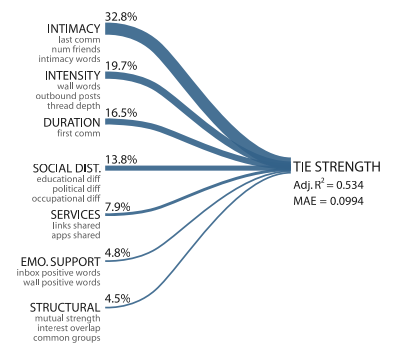
\includegraphics[width=0.7\textwidth]{imgs/composicao-forca.png}
  	\caption{Poder preditivo das sete dimensões da força da conexão
  	\citep{Gilbert2009}}
    \label{fig:forca}
\end{figure}

Esse resultado confirma o papel prescritivo das variáveis estruturais. Não
obstante os resultados, o método de \citet{Gilbert2009} possui restrições quanto
a utilidade em nosso cenário digital. Em primeiro lugar, sua abordagem
supervisionada não escala com a rede e não há estudo sobre o erro induzido pela
amostragem. Em segundo lugar, o tipo de conexão não é direcionado, isto é, ambos
atores conferem o mesmo valor para a relação. Essa simplificação é nociva para o
nosso objetivo de análise de influência, já que a assimetria de influência é
bastante comum, por exemplo, um aluno pode ter grande consideração por um
professor, mas o inverso em pé de igualdade raramente é verdade.

\begin{table} [htbp]
	\setlength{\arrayrulewidth}{2\arrayrulewidth}  % espessura da  linha
	\setlength{\belowcaptionskip}{10pt}  % espaço entre caption e tabela
	\caption{Sumário dos componentes da força da conexão
	\citep{Petroczi2006}} \centering   % tabela centralizada
	\begin{tabular}{| p{4cm} | p{8cm} |}
	\hline
	\textbf{Dimensão} & \textbf{Referências} \\ \hline\hline
	Frequência & \citet{Benassi1999, Blumstein1988, Granovetter1995,
	Marsden1984, MATHEWS1998, Mitchell1987, Perlman1987} \\\hline
	Intimidade & \citet{Blumstein1988, Marsden1984, MATHEWS1998, Mitchell1987,
	Perlman1987}\\\hline 
	Investimento voluntário na relação & \citet{Blumstein1988, Perlman1987}\\\hline
	Aconselhamento dado e recebido & \citet{MATHEWS1998}\\\hline 
	Desejo de companhia & \citet{Blumstein1988, Perlman1987}\\\hline 
	Multiplicade dos contextos em que há interação & \citet{Blumstein1988,
	Granovetter1973, Marsden1984, Perlman1987}\\\hline 
	Duração & \citet{Blumstein1988, Granovetter1973, Marsden1984,
	Perlman1987}\\\hline 
	Reciprocidade & \citet{Blumstein1988, Friedkin1980, Granovetter1973,
	MATHEWS1998, Perlman1987}\\\hline 
	Suporte	emocional (intensidade) & \citet{Blumstein1988, Granovetter1973,
	Mitchell1987, Perlman1987, Wellman1982, Wellman1990}\\\hline
	Confiança & \citet{Granovetter1973, Marsden1984, MATHEWS1998}\\\hline
	Sociabilidade & \citet{Mitchell1987}\\
	\hline
	\end{tabular}
	\label{tab:resumao}
\end{table}

Isso nos leva a reflexão de que, para análise de influência, a utilização de
todas as dimensões da força da conexão pode ser muito restritiva. Uma delas, como
no exemplo já citado, é a dimensão de reciprocidade: um ator com prestígio exerce
grande influência sobre seus admiradores, mas cada admirador individualmente não
consegue exercer influência de igual intensidade sobre ele. Outro exemplo são os
indíviduos de fronteira, que se conectam à periferia de dois grupos; as suas
conexões são fracas, mas exerce grande influência na transferência de
conhecimento entre os grupos. Daí temos que apesar da noção de força de
Granovetter está relacionada com a influência, ela não é condição necessária
\citep{Brown2007}.

Finalmente, nenhuma das soluções estudadas considera a evolução da rede no
tempo. Nesse aspecto algumas pesquisas utilizam fotografias na rede em
momentos diferentes ou agregações das interações por período. A partir daí
utiliza-se modelos probabilísticos \citep{Sarkar2005}, meta-grupos
\citep{Berger-Wolf2006} ou modelos provenientes da psicologia comportamental e da
administração \citep{Brelger2004}. Nenhum deles, entretanto, é combinado com
a teoria da força das conexões para permitir sua aplicação em processos de
mensuração de redes sociais digitais.

A partir de então sugerimos alguns critérios para as ferramentas de mineração
que serão usadas no processo de análise de influência:

\begin{enumerate}
  \item Deve ser não supervisionada para aumentar a chance de escalar com o
  tamanho da rede;
  \item Deve considerar a força das relações na maior quantidade possível de seu
  espectro de componentes. Por tanto, a representação resultante não deve ser
  binária;
  \item Deve também levar em consideração aspectos estruturais da rede como
  transitividade e \emph{brokerage};
  \item Deve ser longitudinal, isto é, incorporar o elemento tempo na análise,
 levando em conta a formação e dissolução de relações, entrada e saída de
 atores;
\end{enumerate}

Uma vez escolhida as ferramentas de mensuração e análise, devemos agora avançar
para o passo seguinte e selecionar quais dados serão usados e se eles são
válidos.


\chapter{Entendendo os dados}
\label{ch:dados}

A primeira crítica que deve ser avaliada é a de que interações digitais não são
um indicador confiável da relação entre dois indivíduos \citep{Clemons2007}. Que
se um amigo virtual não é mais do que um conhecido, não há relação de influência
significativa entre eles. Porém, as pesquisas em redes sociais digitais tem
demonstrado que em sua maior parte, os indivíduos utilizam os meios digitais para
continuar uma relação já existente no mundo \emph{off-line}
\citep{Haythornthwaite2005, Recuero2008, Sassen2002}. Outra vantagem
de ater-se a interação observada é que ela não carrega alguns pontos fracos da
abordagem direta (questionário, entrevista) que é o esquecimento e a omissão das
relações nas respostas (a taxa de erro quando interrogados sobre as interações
que mantiveram chega a 50\% em comparação com a observação) \citep{Mislove2007}.
Mas a vantagem mais óbvia e determinante é o custo, coletar e processar os dados
advindos das interações dos atores no meio digital é muito mais barato que fazer
o mesmo para interações não digitais, na medida em que o tamanho da rede aumenta,
ou mesmo em comparação com entrevistas e questionários. Na casa dos milhões de
membros na rede, qualquer coisa que não seja a primeira opção é atualmente
inviável.

Nessa etapa da mineração, uma vez delineada as técnicas de mensuração, é
necessário escolher quais medianeiros serão utilizados. Recapitulando a definição
de medianeiro: é todo espaço (virtual) em que seja possível 1) definir unicamente
um ator, 2) mapear atores agentes e recepetores a uma interação e suas
propriedades. Alguns exemplos são: salas de batepapo, fórums, lista de discussão,
sites de relacionamentos, sites de compartilhamento de fotos e vídeos. Para cada
medianeiro, o pesquisador pode ter maior ou menor acesso à informação.

Quando a única informação disponível são as publicadas nas páginas da internet
ou outros meios de acesso ao medianeiro, dizemos que sua análise é
\textbf{extrínseca}. A grande maioria dos trabalhos em redes sociais digitais
hoje é feito dessa forma com a confecção de \emph{crawlers}, programas de
computador que percorrem conteúdos \emph{on-line} retirando informações
estruturadas de dados semi-estruturados próprios para o uso humano, como as
\emph{web pages}. Esse tipo de análise é limitada muitas vezes à interação
presumida, já que geralmente através dela é possível saber que um ator publicou
conteúdo na comunidade, mas não quem da comunidade parou para vê-lo.

Quando as informações são coletadas diretamente dos banco de dados do
medianeiro, chamamos essa análise de \textbf{intrínseca}. A análise intrínseca
encerra diversas vantagens, principalmente por ter acesso ao funcionamento da
rede, podendo coletar dados sobre seu uso. São informações como mensagem lidas e
não lidas, tempo usado em cada uma, e que formam um tipo de interação que
chamaremos de \textbf{passiva}.

Porém muitos são os tipos de interação digitais encontradas e enquanto não
tivermos um maior entendimento das suas semelhanças e diferenças, não nos será
possível construir uma abordagem integrada de mensuração. Por uma tipologia das
interações digitais é então que nossa atenção deve agora se voltar.

\section{Por uma tipologia das interações digitais}
\label{sec:tipologia}
O estudo das interações humanas é o objeto das ciências sociais, notadamente, no
contexto micro, da antropologia e etnografia. Somente com a popularização da
internet é que as interações digitais (mediadas por computador) ocuparam maior
destaque nesse meio \citep{Wellman1996, Herring2002}. Uma tipologia inicial
foi proposta por \citet{Burnett2000} e revisada por \citet{Burnett2004}, porém o
seu foco é na distinção entre interações direcionadas e as não-direcionadas para
a aquisição de informação. Nossa tipologia começa dela, mas expande incorporando
conceitos de capital social \citep{Recuero2008} e abrangência
\citep{MARTINEZ2000}.

Podemos dividir as interações digitais por tipo do \textbf{conteúdo},
\textbf{abrangência} e \textbf{intenção}. Os tipos de conteúdos podem ser
divididos em dois grandes grupos: textuais e não textuais. Abrangência consiste
se a interação é individual básica, individual desenvolvida, individual
generalizada ou comum. Finalmente, quanto a intenção podemos classificar a
interação em afirmativa, negativa, conversacional, informativa, conectiva. É
importante ter em mente que as categorias apresentadas não são, de forma alguma,
mutuamente exclusivas, podendo mesmo numa interação singular ser combinadas em
diferentes formas.

\subsection{Por conteúdo}

O tipo do conteúdo da comunicação diz muito sobre o capital social que carrega
\citep{Kim2007}, por exemplo, mensagens síncronas possuem vocabulário mais
limitado, são mais informais e possuem maior carga social fática
\citep{Danet1998, Ko1996, WERRY1996} enquanto que mensagens assíncronas tendem a
ser maiores, mais multifuncionais e linguisticamente complexas
\citep{Herring1999}. De acordo com essas diferenças, mensagens síncronas parecem
ser mais apropriadas para a interação social enquanto que mensagens assíncronas o
são para discussões mais complexas e resolução de problemas.

Também não é nosso objetivo ainda nos aprofundarmos numa análise do discurso
mediado por computador \citep{Herring2001}. A classificação que utilizaremos aqui
usa o conceito de protótipo e por tanto tem expressividade reduzida diante do
surgimento de formas de interação inovadoras \citep{Herring2007}. Porém ela será
suficiente nesse estudo inicial sobre mensuração de redes para a combinação de
diferentes interações. Dividimos inicialmente em duas grandes categorias: textual
e não textual; para cada uma então são listados seus principais protótipos.

\begin{description}
\item[conteúdo textual] Já foi dito o quanto o texto é importante para a
comunicação mediada por computador, mesmo numa época em que o compartilhamento
de vídeos está na moda, o texto, na forma de comentários, continua sendo o
principal móvel das trocas sociais \citep{Herring2002}. São desse tipo:
\begin{itemize}
  \item comentários;
  \item mensagens;
  \item tópicos;
  \item \emph{blogs} e similares;
  \item \emph{microblogging} e similares;
  \item descrições.
\end{itemize}
\item[conteúdo não-textual] Nesse grupo estão relacionados não só as interações
áudiovisuais, mas também as interações ``mudas'' como a formação de conexões
explícitas entre os atores, a classificação mútua dicotômica ou graduada e a
recomendação de conteúdos de terceiros. Exemplos:
\begin{itemize}
  \item fotos;
  \item vídeos;
  \item \emph{links};
  \item conexões explícitas entre os atores;
  \item classificação (\emph{rating}, \emph{ranking}, favoritos);
  \item compartilhamento.
\end{itemize}
\end{description}

\subsection{Por abrangência}

A abrangência define quais são os atores influenciados pela interação, em
outras palavras, os participantes do ``discurso" \citep{Dooley2001}. É através da
abrangência da interação que o processo de mensuração recupera os atores
participantes na conexão mensurada e, por tanto, representa a forma como os
agentes buscam se posicionar na rede como um todo. Essa classificação foi
apresentada uma primeira vez por \citet{MARTINEZ2000}.
\begin{description}
\item[individual básica] Classificam-se neste grupo as interações de caráter
privativo que partem de um ator específico para outro ator. As interações que
tipicamente pertencem a este grupo são as mensagens, os pedidos de conexão e o
compartilhamento de conteúdo do tipo ``\textit{forward}''.
\item[individual desenvolvida] Quando a interação se inicia em um ator e envolve
sua rede imediata de contatos sem estar publicamente disponível para qualquer
membro da rede. São desse grupo, em sua maioria: tópicos de fóruns, fotos,
vídeos, compartilhamentos, microblogging.
\item[individual generalizada] Quando a interação se inicia em um ator e
torna-se pública para todos os atores da rede. Todos os tipos de interação podem
se classificar nesse grupo, depende do grau de livre acesso que a rede
proporciona aos seus membros.
\item[comum] Quando a interação se dá num espaço de igualdade, quer dizer, que
todos podem interagir com todos no mesmo nível, chamamos de interação comum. Um
exemplo claro dessa categoria é as salas de batepapo onde todos podem publicar
mensagens para todos lerem. Listas de discussão também seguem esse modelo.
Um \textit{Blog} em particular não é uma interação comum, na maioria dos casos,
porque só o mantenedor do \textit{blog} pode publicar artigos nele, já o
espaço de comentários do artigo possa ser considerado um espaço comum.
\end{description}

\subsection{Por intenção}

Por último, mas não por menos, temos a intenção com a qual o ator reveste sua
interação. A diferença de intenção não só pode representar mudança significativa
na força da influência, como necessariamente define os possíveis resultados da
interação. Em \citet{Recuero2008} encontramos uma classificação da intenção das
interações, que para o escopo proposto por esse trabalho é suficiente e as divide
em cinco grandes grupos:
\begin{description}
\item[afirmativa] Trata da afirmação de suporte social entre um ator e outro.
Pode ser um comentário positivo relacionado a uma interação prévia do ator
elogiado, uma avaliação positiva, a recomendação do seu conteúdo para outros.
\item[negativa] Quando a interação se dá para depreciar o outro. Pode ser por
comentário, tópicos, mensagens, avaliação negativa.
\item[conversacional] Quando a interação tem caráter pessoal, relacionado a uma
conversação que se inicia ou que está em andamento.
\item[informativo] Quando a intenção é informar um grupo de atores sobre
determinado assunto. Avisos, artigos, propaganda, críticas.
\item[conectivos] Quando a intenção é formar laços explícitos através da rede.
Pedidos para conexão como adicionar à lista de contatos/amigos/etc.
\end{description}
Das três dimensões de classificação da interação, a intenção é certamente a mais
difícil de aferir computacionalmente. Isso por causa da sua característica
subjetiva e que também a torna objeto ideal para a pesquisa qualitativa.
Porém recente evolução da mineração de opinião e análise de sentimentos pode
trazer opções para a análise de intenção no contexto da mensuração das redes
sociais digitais. Para uma compilação dos principais avanços e desafios na
área, nos referimos a \citet{Wilson2005, Ding2007, Pang2008}. Por sua
importância e dificuldade, teremos o cuidado de anotar mensurações de redes
sociais digitais que não levem em consideração a intenção, como
\textbf{análises ingênuas}.

\subsection{Interações passivas}

Para finalizar essa seção sobre interações, falaremos aqui de interações passivas
e comportamentais que podem levar a um maior entendimento de como o ator investe
sua atenção na rede e, por isso mesmo, como se posiciona na rede em relação a
outros atores. Podemos considerar como interação passiva como aquela que não é
necessariamente percebida pelos outros atores além do interagente, nesse tipo
encontram-se todas as interações do ator com o sistema como: mensagens lidas, não
lidas, tempo usado para cada mensagem, perfis visitados, tempo usado na leitura
de outros conteúdos. Essas informações poderiam ser utilizadas numa análise
intrínseca da rede para a concepção de um modelo mais real do interagente quanto
ao dispêndio da atenção.

\subsection{$\bigotimes$ Notação}

Seja $\mathscr{X}$ um medianeiro, existirá um conjunto $\mathscr{L}$ de
interações associado a $\mathscr{X}$. Considere o conjunto $\mathscr{N}$ de
atores envolvidos através do medianeiro $\mathscr{X}$. Temos que para cada
iteração $l_k \in \mathscr{L}$ existe pelo menos um ator $n_i \in \mathscr{N}$
que provocou a interação, chamamos esses atores de agentes ou autores. Também
existe pelos menos um ator $n_j \in \mathscr{N}$ que recebeu a interação,
chamamos esses atores de receptores, audiência ou abrangência. Assim para fins de
notação, sendo $\mathscr{P}(.)$ o conjunto das partes, considere
$A:\mathscr{L}\to\mathscr{P}(\mathscr{N})$ onde $A(l_k)$ é conjunto de autores de
$l_k$. Da mesma forma, faça $R:\mathscr{L}\to\mathscr{P}(\mathscr{N})$ onde
$R(l_k)$ é conjunto de receptores de $l_k$. Nenhuma das duas funções são
inversíveis, porém para economizar a notação definimos
$A^{-1}:\mathscr{N}\to\mathscr{P}(\mathscr{L})$ onde $A^{-1}(n_i)$ é o conjunto
de interações $l$ tal que $n_i \in A(l)$. O mesmo deve ser considerado para
$R^{-1}$.

\section{Uma teoria da atenção como capital social}
\label{sec:teoria_atencao}

Antes de prosseguir para a etapa seguinte na mensuração da rede, gostaríamos de
discutir uma aproximação para a influência entre os atores: atenção como capital
social. Capital social é todo recurso que mantém a rede social
\citep{Coleman1988} e pode ser mobilizado através das conexões
\citep{Gyarmati2004}. Exemplos de capital social são a confiança e o suporte
emocional. Por esta razão, uma outra forma de chamar as dimensões de força de
\citeauthor{Granovetter1973} é de capital social, i.e., quanto maior o fluxo de
capital social que a conexão suporta, maior será a sua força. Mostraremos que a
atenção não só atende a definição de capital social, como se aproxima mais do
conceito de influência e, certamente, é mais fácil de medir.

Foi o vencedor do prémio nobel, o economista Herbert Simon, que disse:

\begin{quote}{\citep{Simon1996}}\emph{O que informação consome é bastante óbvio:
consome a atenção de seus receptores. Por isso, uma fartura de informação
provoca uma pobreza de atenção.}
\end{quote}

Vivemos em uma era de riqueza de informação e por esta razão estamos em escassez
de atenção \citep{Goldhaber1997}. Atenção é vista atualmente como \textbf{o} mais
importante recursos para as organizações \citep{Davenport2001}. Ela também assume
papel crucial na formação e manutenção de relacionamentos e como é um recurso
limitado, o mais comum é que cada um invista nas relações que percebam ser mais
importantes \citep{Dindia1993}. Por esta razão a atenção satisfaz os critérios de
capital social, a saber 1) contribuir na manutenção da rede, 2) pode ser
mobilizada através das conexões. Vários estudos consideram a atenção como a nova
economia na internet, através de comentários, classificações positivas e
\textit{profiles} \citep{Humphreys2009, Wu2009, Skageby2009}. Nessa economia nós
temos ``celebridades'' e ``fãs'', muito similar ao que encontramos no contexto da
influência.

Na verdade somente o ato de prestar atenção já é receber influência per si,
independentemente das futuras escolhas do receptor. Em uma pesquisa em Parma, na
Itália, por volta de 1991, neurocientistas conectaram cabos ao cérebro de macacos
de forma que o computador reconhecia pelo padrão de ativação dos neurônios quando
ele levava um amendoin à boca. Não obstante a ativação fosse registrada
eletronicamente, eles também ligaram o aparato a um auto-falante de forma que
mesmo estando distantes soubessem quando o evento acontecia. Quando um aluno
passou pelo laboratório e levou uma banana à boca, o alarme soou. Porém o macaco
não estava fazendo nada além de observar o estudante. Estava claro que a atenção
no gesto do estudante disparava o cérebro a reproduzir (em sua mente) o movimento
como se fosse seu (\citealt{Rizzolatti1996}; apud \citealt{Goldhaber2006}).

Resta-nos saber como mediremos a atenção. Ora, em qualquer interação o que é
trocado em primeiro lugar entre o agente e os receptores é atenção. A atenção
flui não só do receptor para o agente ao receber a ``mensagem'', no que chamamos
de atenção \textbf{direta}, mas também do agente para os receptores, por a ter
preparado e comunicado, que chamamos de atenção \textbf{residual}
\citep{Goldhaber1997}. Apesar de que em quantias bem menores proporcionalmente,
porque o que cada receptor recebe é uma atenção ilusória, é uma fração da
atenção do agente e que o satisfaz de alguma forma na interação de modo que para
ele parece um bom negócio continuar retribuindo-a com a sua. Mas como essa
atenção se relaciona com as dimensões da força de Granovetter? Para responder
essa questão precisaremos usar nossa tipologia da interação.

Em primeiro lugar, frequência e duração são dimensões temporais que são
recuperadas a partir do tratamento longitudinal da rede. A frequencia das
interações e data do começo delas são métricas simples de colher e que contribuem
para o total da força. Quanto a intimidade, podemos verificar que a
depender da abrangência teremos espaço para maior ou menor intimidade, ou seja, quando mais
restrito a abrangência mais íntima a interação, sendo a mensagem de pessoa a
pessoa a forma mais íntima possível. Quanto a carga emocional, mesmo não tendo à
disposição meios de análise de sentimento, sabemos que as interações que mais nos
chamam atenção são as que possuem carga emocional \citep{Davenport2001}. Daí
podemos aproximar a dimensão de suporte emocional por uma combinação da de
duração, frequência e intensidade.

Para finalizar nossa consideração sobre a atenção como capital social, é
importante mencionar que a atenção não é direcionada apenas sobre um foco, mas
sobre o contexto. Isto quer dizer que alguns indivíduos podem receber atenção
indiretamente ao serem citados, por intermediarem a interação ou por
simplesmente fazer parte do contexto de alguma forma. Essa atenção chamamos de
\textbf{transitiva}.

\subsection{$\bigotimes$ Formalização}

Considere dois atores $i$ e $j \in \mathscr{N}$; se $\mathscr{X}$ é um medianeiro
para $\mathscr{N}$ com um conjunto de interações $\mathscr{L}$, considere também
$l$ uma interação de $\mathscr{L}$. Se $i \in A(l)$ e $j \in R(l)$ então existe
uma atenção direta $v_{jil}\neq0$ de $j$ para $i$ e uma atenção residual de $i$
para $j$ expressa como $\dot{v}_{ijl}\neq0$. Usaremos o símbolo $+$ em um índice
quando queremos dizer que trata-se do somatório sobre todo o seu conjunto, alguns
exemplos: $v_{i+l} = \sum_{j \in \mathscr{N}}v_{ijl}$ representa toda a atenção
direta investida por $i$ na interação $l$; $v_{ij+} = \sum_{l \in
\mathscr{L}}v_{ijl}$, toda atenção direta cedida de $i$ para $j$ considerando
todas as interações; e $v_{++l} = \sum_{i \in \mathscr{N}}\sum_{j \in
\mathscr{N}}v_{ijl}$, toda a atenção direta cedida na rede através da interação
$l$.

Algumas restrições são óbvias, como o total de atenção investida em um ator
qualquer é: $v_{i++} + \dot{v}_{i++} = c, \forall i \in \mathscr{N}$. Essa
restrição, no entanto, não se sustenta quando só temos as interações da rede
para avaliar já que representam apenas uma fração da atenção total do ator.

Para definir a atenção transitiva é necessário primeiro estabelecer a relação
$T:\mathscr{L}\to\mathscr{L}$ tal que se $l$ e $q \in \mathscr{L}$ e uma faz
parte do contexto da outra, isto é, estão encadeadas, então $q \in T(l)$ se $q$
veio antes. Dizemos que há atenção transitiva $\widetriangle{v}_{ijl}$ se há um
caminho entre $i$ e $j$ através de $v$, isto é, se $i \in R(l)$ e $j \in A(q)$
para algum $q \in T(l)$. Exemplos de interações encadeadas são comentários de
\emph{posts}, \emph{threads} em fóruns e recomendação de conteúdo.

\chapter{Preparação dos dados}
\label{ch:preparacao}

Na etapa de preparação dos dados, a representação da rede propriamente dita é
mensurada. Apesar dessa mensuração ser por si só um processo de mineração de
dados, apresentamos como pertencente à etapa de preparação porque o intento final
é a análise de influência que vai ser feita em cima da rede, não a rede em si.
Neste capítulo, portanto, apresentaremos algumas técnicas de mineração de dados
para a mensuração da rede, as dificuldades existentes quando se utiliza
aprendizagem de máquina e faremos algumas considerações sobre técnicas para a
escolha dos dados mais relevantes.

Trataremos aqui principalmente de mensurações da rede, que é a primeira parte do
processo de análise de influência. A mensuração, por sua vez, se divide em dois
momentos: dados \textbf{brutos} e dados \textbf{compilados}. No seu estado bruto,
a rede guarda os dados como se lhe apresentam através dos medianeiros, por
exemplo: quantidade de interações, tamanho das interações, classificações usadas,
data da interação, etc. Esse processo por si so é trabalhoso, pois devemos ter o
cuidado de guardar não só as interações, mas as propriedades relacionadas a elas.
Também é comum a formação de hipergrafos, isto é, grafos onde os atores são
agrupados por alguma relação \citep{Breiger1974, Seidman1978}. Um exemplo
claro de hipergrafo é a representação formada a partir da afiliação dos atores à
comunidades, contudo, a rigor, toda interação particiona o grafo em um
subconjunto.

\section{Exemplo de hipergrafo}

Considere dois medianeiros $A$ e $B$ que mediam o mesmo conjunto de
atores $\mathscr{N} = \{n_1, n_2, n_3\}$. Em $A$, coletamos duas interações
$i_1$ e $i_2$. O ator $n_1$ é o autor de ambas interações. O ator $n_2$ é o
receptor da interação $i_1$ e o ator $n_3$ é o receptor da interação $i_2$. Se
construirmos uma matriz de adjacência e um hipergrafo a partir do medianeiro $A$
teremos o resultado apresentado na \figref{fig:hiperg1}:

\begin{figure}[htb]
  \centering
  \begin{minipage}[c]{0.48\textwidth}
    \centering
    \begin{array}{c | c c c}
	& n_1 & n_2 & n_3 \\ \hline
	n_1&0&1&1\\
	n_2&0&0&0\\
	n_3&0&0&0\\
	\end{array}
  \end{minipage}
  \begin{minipage}[c]{0.38\textwidth}
    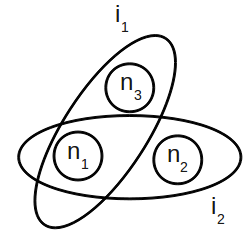
\includegraphics[width=\textwidth]{imgs/hipergraf1v.png}
  \end{minipage}
  \caption{hipergrafo de $A$ -- três atores, duas
  interações.}\label{fig:hiperg1}
\end{figure}

Já em $B$ temos apenas uma interação, $i_3$, cujos receptores são $n_2$ e $n_3$.
Se construirmos sua matriz de adjacência, ela será igual à de $A$ porem os
hipergrafos demonstram grande diferença, já que em $B$ o ator $n_1$ alcançou
$n_2$ e $n_3$ com uma única interação.

\begin{figure}[htb]
  \centering
  \begin{minipage}[c]{0.48\textwidth}
    \centering
    \begin{array}{c | c c c}
	& n_1 & n_2 & n_3 \\ \hline
	n_1&0&1&1\\
	n_2&0&0&0\\
	n_3&0&0&0\\
	\end{array}
  \end{minipage}
  \begin{minipage}[c]{0.28\textwidth}
    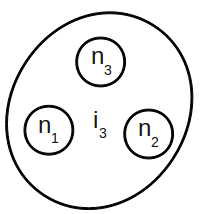
\includegraphics[width=\textwidth]{imgs/hipergraf2v.png}
  \end{minipage}
  \caption{hipergrafo de $B$ -- três atores, uma
  interação.}\label{fig:hiperg2}
\end{figure}

Nenhum das abordagens citadas no \chapref{ch:dominio} consideram o aspecto de
hipergrafo das interações. Seria necessário adaptar as técnicas de análise de
influência se quisermos considerar um ator que influencia muitos em uma única
interação de outro que o faz através de muitas interações separadas. Tendo isso
em mente, partimos para as técnicas de mensuração em si.

\section{Interações não-textuais}

Uma possível abordagem foi a citada no exemplo acima, a da ausência ou presença
de interação. Ela foi usada por \citet{Xiang2010} e simplifica a representação
em uma rede dicotômica. Outras possibilidades está em contar a quantidade de
interações ocorridas, a frequência por período, a idade da primeira interação, a
presença em comunidades comuns, similaridade de perfil, etc. De forma geral
podemos criar a rede por:

\begin{itemize}
\item Intensidade/Quantidade
\item Frequência
\item Presença/Ausência
\item Properidade única (e.g., Longevidade)
\item Similaridade
\end{itemize}

Cada uma dessas apresenta apenas uma dimensão da relação, de forma que para o
mesmo medianeiro mais de uma representação pode ser mensurada a partir de
diferentes formas de agregação. Outras representações ainda podem ser criadas a
partir da combinação de mensurações diferentes, por exemplo: intensidade x
frequência, longevidade x similaridade. Deve-se ter um cuidado extra no uso de
agregações porque podem introduzir correlações espúrias no conjunto de dados,
levando a erros do tipo I (falso positivo) e tipo II (falso negativo), pois a
agregação mascara quais elementos estão correlacionados de fato
\citep{Jensen2003}. Não existe forma correta de escolher as agregações, porém
veremos mais adiante como poderemos diminuir o impacto disso no processo como um
todo.

No final, teremos uma ou mais representações da rede para cada tipo de
medianeiro, que por diferença de natureza não são facilmente integráveis.
Contando, porém, com uma análise intrínseca dos medianeiros, poríamos apostar
numa integração pela teoria da atenção. Apesar de que tempo gasto não se traduz
diretamente em atenção dispendida, poderíamos mensurar o tempo que o usuário do
medianeiro empregou em cada interação e daí inferir uma valor em unidade única:
atenção \citep{Davenport2001}. Com isso teríamos o tempo empregado na
visualização de um vídeo, de uma foto como estimativa da atenção. Essa análise
nem sempre é possível e mesmo que seja, há interações que são naturalmente
difíceis de integrar, como as avaliações (\emph{ratings}, \emph{rankings}). As
avaliações tomam sempre o mesmo tempo (o do clique do mouse) e seu conteúdo é
totalmente ``emocional'', isto é, polarizado entre positivo e negativo. Caso seja
utilizado técnicas de análise de sentimentos para as outras interações, então
talvez as avaliações possam ser integradas pela dimensão emocional da força da
relação. Por outro lado, avaliações são excelentes opções para a utilização como
grupo de teste para algoritmos de aprendizagem de máquina ``supervisionados''.

\section{Interações textuais}

Na seção anterior investigamos as relações não-textuais, agora vamos nos deter
nas textuais. Primeiramente, intentamos com essa divisão alcançar uma
consequência prática: a integração de diversas interações numa só rede. A rede
que vamos construir é valorada, isto é, as conexões possuem um peso na forma de
um número real dentro de um intervalo. Ao contrário de redes binárias, as redes
valoradas proporcionam um indicativo da \textbf{força} da conexão entre os
atores.

Dentro de uma teoria da atenção como capital social, devemos então nos voltar
para a afirmação de que laços por onde trafegam muitos recursos são laços fortes
e o contrário também é verdade. Em cada interação na rede, como vimos, tem um
ator-agente que inicia a interação e um grupo de abrangência, que chamaremos de
atores-receptores, que é afetado por ela. Com esse modelo, podemos estimar que
os receptores cedem atenção para o agente e a recíproca também é verdadeira,
pois o agente escolheu interagir com este grupo e essa escolha já é um
indicativo de atenção cedida.

Idealmente, essa atenção poderia ser mensurada a partir do tempo empregado pelos
atores na interação, mas quase nunca essa informação está disponível. Por esta
razão, sugerimos a quantidade de palavras na interação textual como uma
estimativa para a quantidade de atenção trocada na interação. A sugestão advém
naturalmente do fato de que quanto maior o texto, mais tempo é empregado na sua
leitura, possivelmente mais recursos cognitivos também serão empregados para a
sua apreensão. Isso nem sempre é verdade para todos os textos, ou tipos de
textos, mas restringindo nosso escopo para comunidades virtuais de amigos e/ou
comunidades de prática \citep{Lave1991, Lave1991a}, acreditamos ser esse
um bom ponto de partida.

Outro cuidado necessário é na determinação se de fato a interação foi percebida
pelos receptores. Na maioria das vezes essa determinação é inviável, aumentando
a incerteza do modelo. Entretanto, um recurso simples que pode ser utilizado é
procurar por interações encadeadas, isto é, quando uma interação posterior é 
reação a outra anterior. Por exemplo, quando uma mensagem é respondida, um texto
é comentado, um conteúdo é recomendado, em todos esses casos podemos avaliar que
o agente que reagiu não só percebeu a interação do agente anterior, como se deu
o trabalho de responder. Em verdade, para interações que normalmente se
encadeiam como \emph{threads} de fórums ou listas de discussão, podemos
considerar a resposta como um sinal de atenção não só para com o participante
imediatamente anterior, mas para vários antes dele que de certa forma
influenciaram na resposta atual.

Assim, podemos construir uma rede onde os nós são os atores e os laços é o
somatório da atenção trocada pelos mesmos. Quanto mais textos de um ator $a$
lidos, respondidos, recomendados, avaliados por um ator $b$, maior será a força
da relação direcionada de $b$ para $a$. Quanto mais conteúdo um ator $a$ publica
para um determinado público, mais forte também será sua relação direcionada
com o mesmo. Tal rede, por tanto, integraria insumos de diversos tipos de
interação mensurados, desde que sejam de conteúdo textual.

\subsection{$\bigotimes$ Formalização}
\label{sec:formalizacao}
Para a formalização dessa métrica, vamos usar um exemplo prático. Em um fórum
qualquer, vamos tomar um tópico para nosso exemplo. O fórum é o
\textbf{medianeiro}, os membros assinantes do fórum os \textbf{atores}. O tipo de
interação é \textbf{textual} quanto ao conteúdo, \textbf{comum} quanto a
abrangência e nossa análise será \textbf{ingênua}, isto é, não consideraremos a
intenção. Revisando:
\begin{itemize}
  \item $\mathscr{N}$ o conjunto de $N$ atores e o $i$-ésimo ator é $n_i$,
  $i=1,2,\ldots,N$;
  \item $\mathscr{L}$ o conjunto de $L$ tópicos do fórum e o $k$-ésimo
  tópico é $l_k$, $k=1,2,\ldots,L$;
  \item $A:\mathscr{L}\to \mathscr{N}$ tal que $A(l_k)$ seja o
  autor do tópico $l_k$, a função $A$ não é inversível, dado que um ator pode
  ser autor de mais de um tópico, porém considere a função
  $A^{-1}:\mathscr{N}\to \mathscr{P}(\mathscr{L})$ tal que $A^{-1}(n_i) = \{x
  \in \mathscr{L}|A(x) = n_i\}$ representando o conjunto de tópicos escritos
  pelo ator;
  \item $R:\mathscr{L}\to \mathscr{P}(\mathscr{N})$ tal que todo $x \in R(l_k)$
  é um receptor de $l_k$, considere também o conjunto de tópicos recebidos por
  um ator como sendo $R^{-1}:\mathscr{N}\to \mathscr{P}(\mathscr{L})$ tal que
  $R^{-1}(n_i) = \{x \in \mathscr{L}|n_i\in R(x)\}$;
  \item Se $x \in \mathscr{L}$, $|x|$ é a quantidade de palavras de $x$, para
  todos os outros casos, quando aplicável, é a cardinalidade do conjunto;
\end{itemize}

Definimos a atenção total cedida de $n_i$ para $n_j$, $\vec{v}_{ij+}$
como a soma de suas atenções diretas $v_{ij+}$, residuais $\dot{v}_{ij+}$ e
transitivas $\widetriangle{v}_{ij+}$. A atenção direta é aquela formada quando
$n_i$ é receptor de $n_j$ numa interação $l_k$ e definimos como:

\begin{equation}
\label{def:atedireta}
v_{ijk} = \alpha |l_k| 
\end{equation}

A atenção residual é cedida quando $n_j$ esta na abrangência da interação $l_k$
cujo autor é $n_i$ e definimos como:

\begin{equation}
\label{def:ateresidual}
\dot{v}_{ijk} = \beta |l_k|
\end{equation}

A atenção transitiva é aquela $n_j$ recebe de $n_i$ se este é o autor de algum
tópico $l_k$ que responde a um anterior de autoria do primeiro. Para definirmos
$\widetriangle{v}$ devemos antes modelar o encadeamento dos tópicos. Seja
$T:\mathscr{L}\to \mathscr{L}\cup\{\varnothing\}$, se $l_h=T(l_k)$ então
$l_k$ é uma resposta a $l_h$, se $l_k$ é a mensagem que iniciou o tópico então
$T(l_k)=\varnothing$. Agora faça $T^*:\mathscr{L}\to\mathscr{P}(\mathscr{L})$:

\begin{equation}
\label{def:thread}
T^*(l_k) = \left\{ \begin{array}{l l} \varnothing &\quad\text{se
$T(l_k)=\varnothing$}\\ \{T(l_k)\} \cup T^*(T(l_k)) &\quad\text{em todo outro
caso}\end{array} \right.
\end{equation}

Daí temos que $T^*(l_k)$ é conjunto de todas as $m$ mensagens anteriores na
\emph{thread} de $l_k$ e podemos definir uma sequência $t^*_{kq}$, onde
$q=1,2,\ldots,m$, sobre esse conjunto considerando a ordenação trivial: $a > b
\iff a\in T^*(b)$. Dessa forma $l_k$ é uma resposta a $t^*_{k1}$, que por sua
vez responde a $t^*_{k2}$ e assim sucessivamente até a mensagem inicial. Levando em
consideração a \defref{def:thread}, definimos a atenção transitiva como:

\begin{equation}
\label{def:atetransitiva}
\begin{array}{ l l }
\widetriangle{v}_{ijk} = \sum_{q}(1-\alpha)\gamma^q|t^*_{kq}| 
&, q \in \{x | A(t^*_{kx}) = n_j\}
\end{array}
\end{equation}

A partir das Definições em \ref{def:atedireta}, \ref{def:ateresidual} e
\ref{def:atetransitiva} podemos calcular a atenção total entre $n_i$ e $n_j$
como:

\begin{equation}
\label{def:atetotal}
\vec{v}_{ij+} = E(n_i)\frac{v_{ij+} + \dot{v}_{ij+} +
\widetriangle{v}_{ij+}}{v_{i++} + \dot{v}_{i++} + \widetriangle{v}_{i++}}
\end{equation}

Evidentemente, este é um modelo exploratório para a mensuração de redes a partir
de interações textuais sob um ponto de vista generalista. Nesse sentido há muito
espaço para aperfeiçoamento dentro do campo experimental. Para finalizar,
devemos fazer mais algumas considerações:
\begin{itemize}
  \item $\vec{v}_{ij+}$ tem sua soma normalizada devido ao limite de atenção
  natural de cada um;
  \item Porém, cada pessoa dedica quantidades diferentes de atenção total aos
  medianeiros analisados, de forma que seria simplório normalizar todos em 1.
  Por esta razão, cada ator tem a soma de suas atenções distribuídas na rede
  normalizada em um fator $E(n_i)$ que indica o seu grau de atividade na rede.
  Esse fator, \emph{a priori} será sempre relativo e caso o escolhamos como
  sendo a razão do total de atenção cedido pelo ator sobre a maior atenção
  medida, teremos uma normalização absoluta para toda a rede baseada no seu
  máximo. O que pode não ser a melhor escolha, pois idealmente a restrição de
  atenção deve servir para reduzir a variância da força das conexões na rede;
  \item O parâmetro $\gamma$ representa a força da influência de mensagens
  antigas na $thread$ sobre um determinado ator em sua participação atual. Por
  esta razão $0 \leq \gamma \leq 1$, sendo que $\gamma=0$ anula toda a atenção
  transitiva e $\gamma=1$ considera todas as mensagens anteriores como sendo
  igualmente influentes na mensagem atual;
  \item O parâmetro $\beta$ representa a atenção recíproca do agente para os
  seus recptores, também varia de 0 a 1, sendo que $\beta=0$ anula a atenção
  residual da composição e $\beta=1$ indica que o autor da mensagem cedeu
  individualmente a cada receptor tanto quanto este para com ele. Um valor
  interessante para $\beta$ é o inverso da quantidade de atores na abrangência
  da interação em contexto, isto é, $\beta=^1/_{|A(l_k)|}$. Assim, o autor cede
  uma fração igual para cada receptor que é tão menor quanto maior for seu
  público. Essa proporção também satisfaz a dimensão de intimidade da força da
  conexão, já que interações mais íntimas (menor abrangência) mobilizam maior
  atenção;
  \item O parâmetro $\alpha$ representa o quão certos estamos de que a interação
  foi recebida integralmente pelo receptor. A sua escolha depende de diversos
  fatores da análise empregada sobre os medianeiros, pois que para cada caso
  poderemos (ou não) averiguar a atenção média cedida por um ator a uma
  interação que lhe chega qualquer. Se $\alpha=0$ indica que caso o receptor não
  tenha respondido à interação de alguma forma, ele não foi influenciado por
  ela. $\alpha=1$ retira qualquer valor do fato do ator ter respondido ou não
  determinada mensagem, igualando os dois casos. Em geral, mesmo que tenhamos o
  indicativo de que o receptor recebeu a interação, é interessante manter um
  valor de $\alpha$ diferente dos extremos para premiar a relação entre atores
  que se respondem. O parâmetro $\alpha$ também pode ser visto no contexto da
  dimensão de reciprocidade da força da conexão, já que quanto menor o $\alpha$
  mais forte será proporcionalmente as conexões em que houveram reciprocidade.
\end{itemize}

\section{Critérios de escolha da representação}
\label{sec:criterios}
Qual a rede ideal para a análise de influência? Não há resposta objetiva para
essa pergunta. Cada rede é uma representação de um fenômeno social que vai além
das ferramentas, mesmo sendo capaz de coletar e integrar todas as interações
digitais, as pessoas ainda vão ser capazes de tomar café juntas e nossa visão
será apenas parcial. Sendo assim, é evidente que cada representação mensurada é
uma parte da informação e, portanto, capaz de descrever aspectos diferentes ou
não do fenômeno. São essas variações entre as representações de redes que
chamaremos de \textbf{critérios de escolha}.

Para enteder sua utilidade, um exemplo: imaginemos que ao final da análise
tenhamos duas ou mais representações da rede: uma textual e algumas não textuais.
Para cada uma encontramos valores diferentes de proeminência, então qual usar?
Colocando de outra forma, quanto de informação estarei perdendo caso considere
apenas uma delas?

A seleção de característica (\emph{feature selection}), na aprendizagem de
máquina, é a tarefa de escolher quais variáveis serão consideradas no treinamento
do sistema de forma a obter a melhor aproximação do modelo \citep{Jain1997,
Blum1997, Jain2000}. De forma similar devemos ser capazes de selecionar redes que
maximizem nossa análise de influência. Recentemente, \citet{Peng2005} sugere que
as variáveis sejam escolhidas de forma a maximizar a relevância e reduzir a
redundância, mRMR (\emph{minimal-redundancy-maximal-relevance}). No nosso caso,
não conhecemos o modelo da rede \emph{a priori} e a inferência é
não-supervisionada. Por isso, não temos como avaliar a relevância de uma rede em
relação a outra, todas são relevantes. Poderíamos considerar que redes que não
demonstrem características de redes sociais poderiam ser vistas como fortemente
enviesadas e por isso de baixa relevância, a saber: diâmetro pequeno (\emph{small
world}) \citep{Milgram1967, Watts1998}, poucos muito conectados e muitos pouco
conectados (\emph{power-law}) \citep{Liljeros2001, Mitzenmacher2004} e atores com
muitas conexões tendem a estar conectados uns aos outros (\emph{scale-free})
\citep{Li2005}.

Por outro lado, a redundância da informação nos ajudará a separar as
representações importantes das que não acrescentam informação substancial, ou
seja, são redundantes. Sendo assim, nosso objetivo é formular alguns critérios
de escolha, de modo que tenhamos em mãos o conjunto de representações
minimamente redundante.

\subsection{$\bigotimes$ Mínima redundância}

Dada uma entrada de dados $D$, composta de $N$ amostras e $M$
características $X=\{x_i, i=1,\ldots,M\}$, dizemos que um subconjunto $S
\subseteq X$ de $m$ características $\{x_i\}$ é mínimamente redundante se atende
a condição:

\begin{equation}
\label{def:min_redun}
\min R(S), R = \frac{1}{|S|^2}\sum_{x_i, x_j \in S}I(x_i;x_j)
\end{equation}

$I(.)$ é a função de informação mútua e que mede uma forma de dependência entre
duas variáveis aleatórias. Dado duas variáveis aleatórias discretas, $X$ e $Y$
definimos a informação mútua de ambas como:

\begin{equation}
\label{def:inf_mutua}
I(X;Y) = \sum_{x\in X}\sum_{y\in Y}p(x,y)\log \frac{p(x,y)}{p(x)p(y)}
\end{equation}

Um dos inconvenientes de utilizar a função de mútua informação como definida é
que no caso de redes sociais, cada conexão pode ser considerada como uma
variável aleatória de resultados possíveis $\{0,1\}$ quando binária, ou um
intervalo definido. Se assim for, não podemos dizer muito da probabilidade da
relação existir ou não (por enquanto). Se por outro lado considerarmos a
variável como sendo a prossibilidade da presença da relação (para simplificar) e
cada par de atores uma amostra dessa variável, então estaremos encontrando
dependência ou correlação sobre a densidade da rede apenas, deixando de lado
importante padrões estruturais como a transitividade e a reciprocidade. Por esta
razão, precisamos adaptar nossa função de mútua informação para considerar as
peculiaridades das redes sociais. 

\subsection{Redundância das conexões}

Uma conexão é redundante quando pode ser encontrada em mais de uma rede. Mais do
que isso, duas redes são redundantes quando além de compartilhar conexões também
compartilham determinados padrões como triângulos e subgrupos. As duas
famílias de ferramentas para acessar essa similaridade estrutural mais
desenvolvidas na literatura são: gráficos aleatórios exponenciais e procedimento
de atribuição quadrática, respectivamente $p*$ (\emph{exponential random
graphs}) e \emph{QAP} (\emph{quadratic assignment procedure}).

\subsection{$\bigotimes$ Redes discretas e/ou esparsas}

O primeiro é mais apropriado para redes binárias ou com valores discretos
\citep{Dekker2007}. Consiste em criar um modelo exponencial para a criação de
grafos aleatórios a partir de um conjunto de parâmetros relacionados a
\textbf{configurações} de interesse \citep{ROBINS2007a}. Uma configuração pode
ser desde a presença de uma conexão, até a quantidade de k-triângulos e outros
padrões mais complexos. Cada configuração tem um parâmetro relacionado que pode
ser negativo, indicando que a rede tem tendência inversa à presença daquela
configuração, nula representando a indiferença e positiva para uma tendência de
mesmo modo. Assim sendo, cada parâmetro pode ser visto como tendências da rede em
relação a, por exemplo: densidade, reciprocidade e transitividade da rede quando
suas configurações relativas são respectivamente a presença de conexões, a
mutualidade das relações e a presença de triângulos.

Modelos exponenciais de gráficos aleatórios tem a seguinte forma geral:

\begin{equation}
\label{def:p_star_geral}
\Pr(\textbf{Y} = \textbf{y})
=\left(\frac{1}{k}\right)\exp\left\{\sum_A\eta_Ag_A(\textbf{y})\right\}
\end{equation}

Onde (i) o somatório é sobre todas as configurações procuradas em \textbf{y};
(ii) $\eta_A$ é o parâmetro relacionado à configuração $A$; (iii)
$g_A(\textbf{y})=1$ se a configuração é observada em \textbf{y}, ou 0 de outra
forma; (iv) $k$ é uma constante de normalização que garante que
a \defref{def:p_star_geral} seja uma distribuição de probabilidades. O vetor de
parâmetros $\eta$ é estimado para o grafo a ser modelado, procurando maximizar
a sua probabilidade, iterativamente a partir de simulações com o método Monte
Carlo (\emph{Markov chain Monte Carlo maximum likelihood estimation})
\citep{ROBINS2007b, Snijders2006}.

Voltando ao problema de minimizar a redundância, podemos considerar o vetor
$\eta$ no cálculo de ``informação mútua'' entre as redes, no sentido de que redes
que possuem a mesma informação compartilham conexões e tendências similares ao
aparecimento de padrões estruturais. Derivamos $I_D$ para redes discretas:

\begin{equation}
\label{def:MI_discreto}
I_D(x, y) = sim(x,y) \rho(\eta_x, \eta_y)
\end{equation}

Onde (i) $sim(.)$ é a similaridade de Jaccard (\citealt{Jaccard1912}; apud
\citealt{Berger-Wolf2006}), utilizada para comparar redes sociais e definida como
sendo $\frac{2|x\cap y|}{|x| + |y|}$; (ii) $\rho$ é a correlação de Pearson para
os vetores de parâmetros $\eta$ estimados para $x$ e os estimados para $y$.
Substituindo a \eqnref{def:MI_discreto} na \eqnref{def:min_redun} temos um
modelo para o conjunto de redes discretas com mínima redundância.

\subsection{Redes contínuas densas}

Para rede contínuas, um segundo método pode ser utilizado para calcular a
correlação diretamente. O procedimento de atribuição quadrática (\textit{QAP})
recomenda um modelo linear para a correlação das redes, assim, temos que:

\begin{equation}
\label{def:linear_model_qap}
Y = \alpha X + \epsilon
\end{equation}

A probabilidade de que a correlação encontrada não seja apenas coincidência é
acessada através da permuta das colunas da matriz seguindo algoritmo apropriado
\citep{Anderson2001, Dekker2007}. Não é nosso objetivo nos aprofundar na
especifidades do teste, apenas é pertinente considerarmos a  utilização da
correlação linear $\alpha$ como valor para a informação mútua na
\eqnref{def:min_redun} para redes de valores contínuos densos.

\chapter{Análise da influência}
\label{ch:mineracao}

Após as representações haverem sido mensuradas, chegamos no objetivo de todo o
processo: a análise da influência. Como já foi descrito em seções anteriores, o
entendimento da dinâmica da influência na rede pode facilitar a criação de
campanhas publicitárias virais baseadas no boca-a-boca; a difusão de novas
informações para a comunidade; comunicação interna corporativa; reconhecimento de
especialistas e atores chaves na organização; otimizar buscas
\citep{Kirchhoff2009}. Abordagens recentes focam em modelos probabilísticos e
comportamentais para estimar a dinâmica da influência. Métodos mais tradicionais
de redes sociais voltaram-se para métricas individuais de proeminência para
reconhecer atores chave. Em \citet{Kempe2003} encontramos uma comparação
mostrando que apesar de encontrar um subconjunto ótimo de $n$ atores tal que
maximize a dispersão da influência seja um problema $NP$, algoritmos que
aproximam a solução para modelos dinâmicos superam soluções baseadas na simples
escolha de atores centrais em 18\% (para a métrica de grau) e 40\% (para a
métrica de proximidade). Essas, porém, são métricas tidas na literatura como
sendo de pouca expressividade, o que deixa aberta ainda a possibilidade real da
utilização de métricas de proeminência na análise de influência de redes sociais
digitais.

\section{Sobre Proeminência}
\label{sec:sobre-proem}
Proeminência é a característica dos relacionamentos de um ator que o põe em
evidência para outros atores na rede \citep{Wasserman}. A proeminência,
academicamente, foi separada em dois aspectos: centralidade e prestígio.
Centralidade é como o ator se posiciona na rede, sua interação e envolvimento com
os outros. Prestígio é como os outros atores se posicionam em relação a ele, como
interagem e envolvem-se com ele \citep{Knoke1983}.

Nosso objetivo, identificar atores chaves para processos de influência da rede,
está relacionado diretamente com o conceito de proeminência de forma que podemos
dizer que a usaremos como uma aproximação da influência do ator na transmissão de
conhecimento, inovações e opiniões pela rede. Por estes motivos, cuidado especial
deve ser tomado sobre a forma como calcularemos a proeminência e que
características são esperadas da representação da rede mensurada.

Durante décadas pesquisadores de redes sociais se debruçaram sobre o estudo da
proeminência, desenvolvendo inúmeras métricas que conjuntamente são chamadas de
métricas de centralidade. Quando calculadas considerando os caminhos que
\textbf{saem} do ator, referem-se a sua centralidade propriamente dita. Quando
considera-se os caminhos que \textbf{chegam} no ator, referem-se ao seu
prestígio. Não obstante tenha o comum senso de que essas métricas referem-se de
alguma forma à proeminência do ator, a forma específica tem ficado a cargo de
cada pesquisador que já atribuiu ao seu resultado interpretações como autonomia,
controle, risco, influência, corretagem (\emph{brokerage}), independência,
etc.

\citet{Freeman1979} revisou as métricas existentes à época e as compilou em três
principais centralidades: por grau, por proximidade (\emph{closeness}) e por
intermediação (\emph{betweenness}). Interpretando seus resultados em relação a
quanto o grafo se aproxima de uma estrutura de estrela (\figref{fig:star}),
sua visão de centralização ideal, onde suas métricas alcançam o máximo.

\begin{figure}[h!]
  \centering
    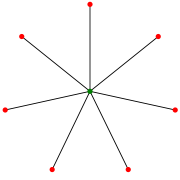
\includegraphics[width=0.3\textwidth]{imgs/star.png}
    \caption{Gráfico estrela}
  	\label{fig:star}
\end{figure}

Recentemente, \citet{Borgatti2006} nos ofereceram uma outra reposta para a
questão: O que as métricas de centralidade medem? E chegaram a conclusão que
todas elas investigam o relacionamento do nó com os possíveis caminhos do grafo.
Em sua tipologia para a classificação das métricas de centralidade, propõem
quatro dimensões: tipo do caminho, propriedade do caminho, tipo do envolvimento e
forma de agregação. Em outras palavras, toda métrica de centralidade é uma forma
de agregar uma propriedade dos caminhos de determinado tipo em que o nó tem um
determinado envolvimento. Das quatro dimensões, duas são de maior importância:
propriedade do caminho e tipo de envolvimento.

\subsection{Tipo de envolvimento} 

O tipo de envolvimento é a dimensão de classificação proposta por Borgatti que
se traduz na maior variância nos resultados. Pode ser de dois tipos: radial ou
medial.

Métricas radiais são as que analisam os caminhos em que o nó está numa das
pontas, ou seja, que saem ou chegam nele. Exemplos de métricas radiais são as
centralidades de grau e proximidade de Freeman. A análise de Borgatti et al veio
confirmar o que as evidências empíricas já sugeriam, que as métricas radiais
representam a parcela de responsabilidade que o nó tem na coesão total da rede e
que, por este motivo, se enfraquecem a medida que a rede não se adequa ao padrão
de núcleo-periferia \citep{Nakao1990}.

Já as ditas mediais analisam os caminhos que passam pelo nó, classificando-o em
seu papel de \emph{gateway} entre partes da rede. O \emph{betweenness} de
Freeman é um exemplo de métrica medial. São mais estáveis em relação à
característica de núcleo-periferia, por outro lado tendem a dar maior importância
a atores que conectam grupos distintos, mas que se encontram na periferia dos
mesmos.

Os dois tipos são complementares e mais de uma métrica devem ser combinadas
(\citealt{Stephenson1989}; apud \citealt{Wasserman}). Pelo fato de que usaremos
métricas radiais de centralidade para estimar a influência do ator na rede, daí
concluímos que quanto mais próximo a representação estiver do modelo de
\textbf{núcleo-periferia}, melhor será a aplicabilidade das métricas radiais de
centralidade.

\subsection{Propriedade do caminho}

Borgatti define dois tipos de propriedade: distância e volume. A
propriedade do tipo distância mais comum é a geodésica que é a quantidade de
arcos presentes no menor caminho entre um ator e outro. Volume refere-se à
quantidade de caminhos entre os nós. As centralidades por grau e
\emph{betweenness} são exemplos de métricas que usam o volume dos caminhos,
enquanto que \emph{closeness} usa distância.

O critério de escolha depende da aplicação. Para o nosso caso, queremos modelar o
efeito da influência entre os pares na transmissão de informação. Nesse sentido,
quanto mais atores próximos estiverem tentando convencer alguém de algo, maior
será sua influência sobre este \citep{Watts2007}. Daí temos, naturalmente, a
preferência sobre métricas relacionadas a volume, no lugar de distância, já que
representa diretamente a quantidade de caminhos que existem entre os nós.

\subsection{Redundância na proeminência}

Vimos no \secref{sec:criterios} como calcular a redundância das conexões entre
representações disponíveis, porém também é interessante observar a relação que há
entre os resultados da análise de cada rede. Para esse fim utilizaremos também a
correlação linear de Pearson entre os vetores de proeminência calculado de forma
que duas redes podem estar positivamente relacionadas, aparentemente
independentes ou negativamente relacionadas. Um critério baseado na proeminência
pode correlacionar redes estruturalmente bastante diferentes, mas que resultam no
sobressaimento dos mesmos atores em termos de importância. Porém, se o objetivo
for minizar a redundância do ponto de vista da ordenação final dos atores por
grau de proeminência para a utilização em outros algoritmos como por exemplo,
escolha de subconjunto ótimo para marketing viral, então talvez este critério
seja o mais apropriado.

\subsection{Relevância na proeminência}
\label{sec:rel_proe}

Quando tudo o que temos é a rede, para medirmos proeminência dos atores
precisamos ser capazes também de medir sua aplicabilidade. Vimos que para alguns
tipos de métricas a rede precisa aprensetar determinado padrão de aglomeração.
Por esta razão, podemos saber \emph{a priori} quando uma representação vai
produzir métricas significativas de proeminência. É sabido que redes sociais são
formadas por diversas comunidades sobrepostas \citep{Palla2005} e por isso uma
representação com alto grau de núcleo/periferia nessas condições é pouco
provável. Uma abordagem seria quebrar a rede em suas comunidades para a partir
daí encontrar os atores centrais de cada uma, existem diversas ferramentas de
decomposição da rede em \emph{k-cliques}, \emph{k-plexes}, \emph{k-cores} para
grafos valorados e direcionados (\citealt{Peay1975, Doreian1969, Freeman1992};
apud \citealt{Wasserman}), mas todas elas tendem a ignorar atores pendentes que
compõem grande parte da periferia.

Um modelo mais interessante para o nosso problema é a chamada comunidade de
prática. A teoria das comunidades de prática não nasceu no meio sociométrico e é
voltada ao estudo da gestão do conhecimento, porém o trabalho de
\citet{Schenkel2002} revisa as características estruturais típicas das
comunidades de prática e sugere quatro delas muito similares ao que estamos
procurando:

\begin{description}
\item[Conectada] A rede possui apenas um componente;
\item[Densa] A média das conexões por ator é alta; o que é considerado
alto varia a depender do tamanho da rede e, por tanto, da periferia;
\item[Compacto] A distância média entre os atores é menor do que o comum para
\emph{small-worlds}, cujo crescimento é logarítmico em relação ao crescimento
da rede;
\item[Núcleo/Periferia] A rede exibe um padrão de núcleo periferia, isto é, alto
grau de \emph{scale-freeness}.
\end{description}

Resta-nos encontrar maneiras de reconhecer essas comunidades e, mais importante,
quais atores a compõem. Comunidades de prática foram definidas como: um grupo de
pessoas informalmente e contextualmente conectadas a uma situação de trabalho em
que estão empregando uma competência comum na perseguição de um objetivo comum
\citep{Wenger1999}. Essas situações de trabalho, no entanto, podem ser
generalizadas para situações que envolvem perícia, conhecimento técnico e por
isso encontraremos comunidades de práticas não apenas no contexto organizacional,
mas entre hobbistas também. O conhecimento em tais comunidades é compartilhado
através de narrativas, conversação, \emph{mentoring} e aprendizagem por
experimentos \citep{Brown1991, Lave1991a}, tais atividades podem ser
transferidas para o meio digital \citep{Hildreth1998, Kimble2001} e deixam
rastros que podem ser mensurados para reconstruir a rede
\citep{Tyler2005, Welser2007}.

É de se esperar, por tanto, que os membros de comunidades de prática se reunam
em torno de focos de interação ondem possam compartilhar histórias, como por
exemplo comunidades virtuais. Para diminuir o ambiguidade do termo, utilizaremos
a palavra \emph{coletividade} quando nos referirmos à comunidade virtual na
qual os atores se afiliam digitalmente. Podemos construir uma rede
de coletividades, onde um nó está ligado a outro se possuem membros em comum,
essa rede é menos sucetível à existência de pendentes e por isso podemos aplicar
algoritmos como os descritos em \citet{Palla2005} para reconhecer coletividades
que se aglomeram em grupos. Essas coletividades poderiam ser usadas depois para
filtrar a rede de atores e verificar se atendem às características de
comunidades de prática, aumentando a relevância da representação para a análise
da influência.

Outra possibilidade é tentar identificar o objetivo ou competência comum que
reúne a comunidade através de mineração de texto. Possibilidades vão desde
encontrar a distância relativa entre os atores baseados em quais palavras
aparecem em seus textos \citep{Reichling2005}, até criar uma ontologia dos termos
propriamente dita e a partir daí estimar uma conexão entre os atores
\citep{Mori2006}. \citet{Spertus2005} propõem o uso da métrica de similaridade
para termos extraídos do texto TF-IDF \citep{Salton1989, Frakes1992} e em
\citet{MATSUO2007} encontramos uma versão aperfeiçoada que diminui a necessidade
de um \emph{corpus} da linguagem. A similaridade, dessa forma, pode indicar uma
homofilia de interesses quando cruzada com as representações mensuradas das
interações, essa homofilia poderia ser usada então para filtrar a rede de atores
e, em verificando as características de comunidades de prática, também vir a
aumentar a relevância da representação na análise da influência.
\chapter{Conclusão e trabalhos futuros}
\label{ch:conclusao}

Nas etapas finais do processo de descoberta do conhecimento, a avaliação e a
utilização, cada domínio fará a aplicação apropriada. Alguns critérios de
relevância para o caso do cálculo de proeminência foram discutidos na
\secref{sec:rel_proe}. Nosso intuito com esse trabalho foi reunir método e
técnicas para um processo pragmático de análise de influência de redes sociais
digitais, oferencendo um passo a passo compreensivo do que pode ser feito, das
dificuldades possíveis e das soluções existentes. Nesse sentido, sentimos que
esse \emph{framework} para a análise de influência em redes está ainda em sua
infância e há muito o que se fazer. Em tópicos gerais, reunimos abaixo os
principais trabalhos futuros:

\begin{itemize}
  \item Considerar a dimensão tempo na dinâmica da rede. Primeiro na
  evolução das conexões, seja através de séries temporais \citep{Snijders1996};
  como intervalos de tempo \citep{Butts2004}; ou como eventos pontuais no tempo
  \citep{Butts2008a}. Depois na evolução da afiliação dos atores a grupos
  através do tempo \citep{Berger-Wolf2006};
  \item Utilizar as informações baseadas em afiliações, estendendo
  modelos \emph{p*} para redes dois-modos (\emph{two-mode network})
  \citep{Field2006}. Em redes de dois-modos há mais de um tipo de nó, no nosso
  caso os atores seriam um tipo, as interações outro tipo. Essa visão
  hiperrelacional da interação permitiria diferenciar padrões de influência do
  tipo ``um para muitos'' dos do tipo ``muitos de um pra um'';
  \item Integrar com modelos estatísticos da economia da atenção para tratar
  fenômenos como a competição pela atenção, sobrecarga de informação e outras
  propriedades de mercado \citep{Falkinger2007}; 
  \item Aplicar o processo de mensuração descrito nesse trabalho a diferentes
  domínios, de forma a melhor avaliar as propriedades de seus parâmetros, sua
  utilidade na análise de influência e facilidade de aplicação.
\end{itemize}

Não obstante, acreditamos que a singular reunião da literatura espalhada sobre
o assunto em um \emph{framework} pragmático facilitará a construção de
ferramentas de mineração apropriadas para o problema. No \appref{ap:estudo} nos
dedicamos a desenvolver essa possibilidade.


\bibliographystyle{natbib}
\addcontentsline{toc}{chapter}{Bibliografia}
\bibliography{references}

% Appendix
\clearpage
\addappheadtotoc
\appendix
\appendixpage
\chapter{Estudo de caso: A.M.I.G.O.S.}
\label{ap:estudo}

Nosso estudo de caso aplica-se sobre um ambiente digital de interação
desenvolvido para a gestão do conhecimento em rede social. Durante o estudo de
caso aplicamos a metodologia proposta no \chapref{ch:kddm} e seu passo a passo
será descrito nas seções \ref{ap:sec:dominio}, \ref{ap:sec:dados},
\ref{ap:sec:preparacao} e \ref{ap:sec:analise}. Nos resultados avaliaremos a
utilidade do método e das ferramentas desenvolvidas no processo.

\section{Entendendo o domínio}
\label{ap:sec:dominio}

Nosso objetivo neste processo de mineração é analisar uma ``fotografia'' do
ambiente digital do a.m.i.g.o.s. e extrair dela um grupo de atores-chaves;
aqueles que se destacam dos demais pelo seu posicionamento ou influência sobre a 
rede. Para darmos prosseguimento a análise, precisamos entender o ambiente e
decidir sobre a ferramenta de análsie que usaremos. Sobre o ambiente temos:

\begin{quote}{\citep{RicardoAraujoCosta2008}}
	Acrônimo de Ambiente Multimídia para Integração de Grupos e Organizações Sociais,
	o a.m.i.g.o.s tem por objetivo prover a infra-estrutura necessária para a criação
	de redes sociais virtuais para os mais diversos fins. Dentre estes, pode-se
	destacar o seu uso para estimular a criação e compartilhamento do conhecimento
	pelos seus diversos membros, podendo estes estarem relacionados a uma organização
	social. Nele é permitida a criação explícita das redes sociais através dos
	usuários e seus contatos. Cada contato é explicitamente adicionado por cada
	usuário, mesmo que dentro de uma mesma organização, e este relacionamento é
	navegável por qualquer outro membro da rede social. Nas próximas linhas são
	apresentadas as principais funcionalidades com suas características e possíveis
	usos.
	\begin{description}
	\item[Perfis] Cada usuário possui um perfil no a.m.i.g.o.s. Este perfil
	consiste de um conjunto de dados preenchidos na forma de cadastro, que definem
	algumas propriedades simples do usuário, como local de residência, idiomas que
	possui conhecimento, endereço de e-mail, identificadores de aplicações de
	mensagem instantânea (Windows Live Messenger, Skype, Google Talk, dentre
	outros), e uma descrição de suas áreas de interesse. Porém a parte mais
	relevante do perfil não é preenchida pelo usuário, e sim inferida pelo
	sistema. [\emph{Para cada usuário, um índice de atividade para a produção e
	consumo de conteúdos também é automaticamente calculado}]
	\item[Histórias] Histórias são destinadas ao registro, compilação e
	apresentação de conhecimentos emergentes entre os participantes da rede.
	Construído de forma gradual, através de contribuições espontâneas ou
	induzidas, qualquer usuário do sistema pode inserir no ambiente suas próprias
	histórias de sucesso ou dilemas, à medida que as considere relevantes para o
	objetivo da rede social. Adicionalmente as histórias podem estar associadas a
	uma ou mais comunidades, o que indica que, apesar do autor ser um usuário em
	específico, o conhecimento construído encontra-se de alguma forma relacionado
	a estas comunidades.

	Cada usuário do sistema poderá, adicionalmente, atuar como um revisor do
	conteúdo inserido por seus pares, avaliando qualitativamente as contribuições
	disponibilizadas neste ambiente. Esta avaliação pode ser realizada de uma das
	duas formas:
	\begin{itemize}
	  \item Adição de comentários que contribuam para a evolução da história,
	  criando-se assim uma história mais rica, com mais participantes e novos
	  conhecimentos. À medida que a história for acrescida de comentários, é criado
	  um diálogo associado ao conhecimento em construção;
	  \item Atribuição de uma nota, variando de uma (1) a cinco (5) estrelas, às
	  histórias que lê. Permitindo que este conhecimento, expresso através de
	  histórias, possa ser apresentado através de um ranking que indique as mais
	  relevantes para os membros daquela rede social.
	\end{itemize}
	\item[Relacionamentos] O a.m.i.g.o.s dá suporte a praticamente todos os
	mecanismos de relacionamentos existentes nas atuais redes sociais. Nele cada
	usuário pode adicionar a sua lista de contatos qualquer outro usuário também
	membro da rede social. Esta lista de contatos pode ser agrupada em grupos,
	facilitando a organização dos contatos pelo seu usuário.
	\item[Comunidades Virtuais] Comunidades podem ser vistas como agregações de
	pessoas com objetivos em comum. O a.m.i.g.o.s dá suporte à criação de
	manutenção de comunidades por parte de seus usuários, podendo estes convidarem
	membros de sua lista de contatos a participar das discussões ou atividades a
	serem realizadas no âmbito da comunidade.

	Cada comunidade possui uma série de mecanismos para a criação e
	compartilhamento do conhecimento. O principal mecanismo de criação e
	compartilhamento do conhecimento é o fórum de discussão, onde os membros da
	comunidade podem iniciar discussões sobre os mais diversos assuntos.

	Um segundo mecanismo de compartilhamento do conhecimento é a associação de
	histórias à comunidade. Esta associação pode ser realizada por qualquer membro
	da comunidade ao criar uma história no sistema. Caso deseje-se, é possível até
	mesmo que a história seja visível apenas pelos membros das comunidades
	relacionadas.
	\item[Recomendações] Como mecanismo de disseminação do conhecimento, o
	a.m.i.g.o.s possui suporte a recomendações. Estas recomendações são sempre
	direcionadas a usuários do sistema e podem ser referentes a histórias,
	comunidades, tópicos de um fórum ou outros usuários. Existem basicamente dois
	tipos de recomendação, uma feita manualmente por um usuário para seus
	contatos, e a outra realizada automaticamente pelo sistema para um usuário a
	partir da probabilidade do interesse deste no conteúdo recomendado.

	Para que a recomendação automática seja possível, o sistema vai montando o
	perfil do usuário à medida que este utiliza o sistema, baseado no que é lido ou
	escrito por ele. Para isto, o sistema faz uso do \emph{Vector Space Model}
	\citep{Barros2002}, varrendo o conteúdo textual disponível em cada elemento,
	calculando então o centróide do conteúdo e conseqüentemente o centróide do
	usuário, este composto pela soma vetorial do centróide de cada um dos seus
	conteúdos. Em seguida o sistema tenta identificar outros usuários ou conteúdos
	com centróides similares, recomendando-os ao usuário em questão sempre que
	esta similaridade for maior que um limiar configurado.
	\end{description}
\end{quote}

\begin{figure}[h!]
  \centering
    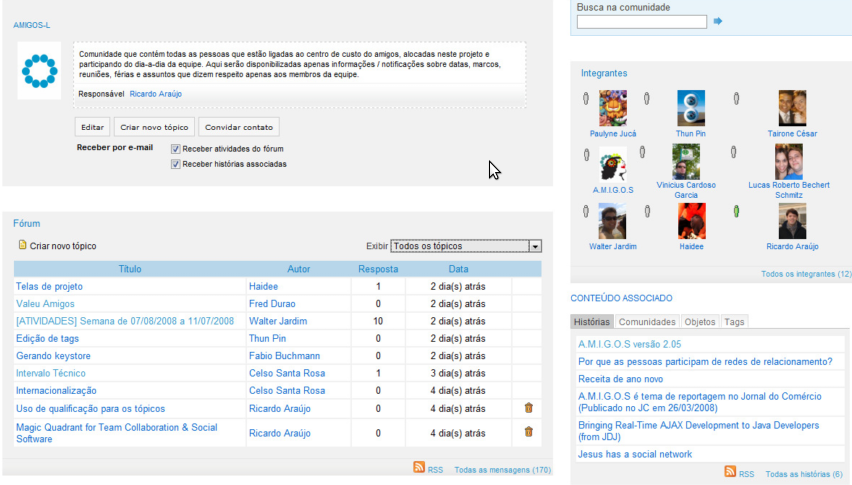
\includegraphics[width=0.7\textwidth]{imgs/screenshot-amigos.png}
  \caption{\emph{Screenshot} da interface do A.M.I.G.O.S.}
    \label{ap:fig:screenshot}
\end{figure}

Considerando os critérios estabelecidos no \chapref{ch:dominio}, temos que a
representação da rede precisa ser não-binária e envolver a maior quantidade de
dimensões da força do laço possível; Por esta razão focaremos nas interações
textuais do a.m.i.g.o.s. usando o conceito de atenção apresentado na
\secref{sec:teoria_atencao}. Para a análise de influência, seguindo a orientação
apresentada na \secref{sec:sobre-proem}, usaremos duas métricas, uma medial e
outra radial; ambas baseadas no volume dos caminhos. As escolhidas foram a
\emph{Flow betweenness} de \citeauthor{Freeman1991} e o poder de
\citeauthor{Bonacich1987}; as razões dessa escolha são a de que atendem aos
critérios de serem sensíveis tanto à estrutura macro da rede, quanto a
configuração local do nó, e também por simplicidade de implementação.

 

\section{Entendendo os Dados}
\label{ap:sec:dados}

Como para os fins desse estudo nos foi cedido o acesso a uma ``fotografia'' do
banco de dados do ambiente, então será uma análise intrínseca; não precisaremos
de \emph{crawlers}. Devido à complexidade de implementar algoritmos de análise de
sentimento, seguiremos uma abordagem ingênua e não consideraremos a intenção da
interação. Como se trata de interações em um contexto organizacional fechado, é
pouco provável que tenhamos disruptores e históricos longos de adversidade, de
forma que podemos considerar que muitas interações entre dois membros é uma bom
indicativo da positividade de suas intenções.

O poder da abordagem apresentada na \secref{sec:teoria_atencao} é a integração
de vários tipos de interação, conquanto sejam textuais. Então utilizaremos
quatro medianeiros textuais reconhecidos no ambiente e classificaremos de
acordo com a tipologia apresentada na \secref{sec:tipologia}:

\begin{description}
\item[Tópicos] são mensagens que \textbf{iniciam} discussões nos fóruns das
comunidades. A abrangência é individual desenvolvida, já que é direcionada aos
membros daquela comunidade apenas.
\item[Respostas] compõem o resto das mensagens nas discussões dos fóruns e
seguem naturalmente os tópicos e umas às outras. A abrangência também é
individual desenvolvida.
\item[Histórias] que são os textos de propósito geral que podem ser visualizados
por qualquer pessoa dentro do sistema, com algumas exceções. A abrangência,
nesse caso, pode ser individual desenvolvida quando relacionada a uma comunidade
apenas ou individual generalizada quando para todo o ambiente.
\item[Comentários] relativos às histórias publicadas. Cada história tem um
espaço público onde qualquer membro pode ler e publicar sua opinião, trata-se
portanto de uma interação de abrangência comum.
\end{description}

É importante denotar a abrangência de cada medianeiro pois que afeta diretamente
o cálculo da atenção residual que cada autor tem com seus leitores. Usaremos o
coeficiente $\beta$ igual ao inverso multiplicativo da quantidade de membros da
abrangência, assim cada autor cede parcelas iguais a sua audiência por cada
interação. Para interações de abrangência generalizada para todo o ambiente, como
é o caso da grande maioria das histórias cadastradas, temos que $\beta=0$, por
tanto, o autor não cede atenção residual para ninguém.

Como nossa anális é intrínseca, pela disposição da informação no banco de dados
podemos saber exatamente qual membro acessou e leu quais tópicos e histórias.
Por esta razão, definimos o coeficiente $\alpha$ da seguinte maneira: 0, caso
não tenha lido; $0.2$, caso tenha. Sendo assim, membros da abrangência que não
leram não cedem atenção ao autor, membros que leram cedem 20\% do total possível
e aqueles que leram e responderam ou comentaram cedem 100\% da atenção.

Fizemos $\gamma=^1/_2$ de forma que a atenção transitiva decai para a metade a
cada elo da \textit{thread}. Infelizmente, mesmo a análise sendo intrínseca, não
tivemos acesos a interações passivas do usuário como, por exemplo, o tempo que
ele passou em cada leitura ou logado no sistema. Dessa forma é complicado
estimar uma função de participação $E(.)$, porém nós podemos considerar o
próprio índice de atividade calculado pelo sistema como aproximação desse
parâmetro.

\section{Preparando os dados}
\label{ap:sec:preparacao}

Segundo \citet{Cios2005}, em torno de 45\% do esforço total empregado no
processo de mineração de dados é usado no passo de preparação dos dados, como
podemos ver na \figref{ap:fig:esforco}. Por esta razão produzimos como
subproduto dessa atividade um \emph{framework} enxuto para a extração e
manipulação dos dados. O banco original é acessível via \emph{SQL}, através do
qual extraímos as interações e armazenamos em outro banco com controle de data
de quando cada interação foi capturada; em cima desse banco criamos uma
estrutura que abstrai a camada de dados da aplicação, permitindo ao pesquisador
utilizar se concentrar na exploração do grafo.

\begin{figure}[h!]
  \centering
    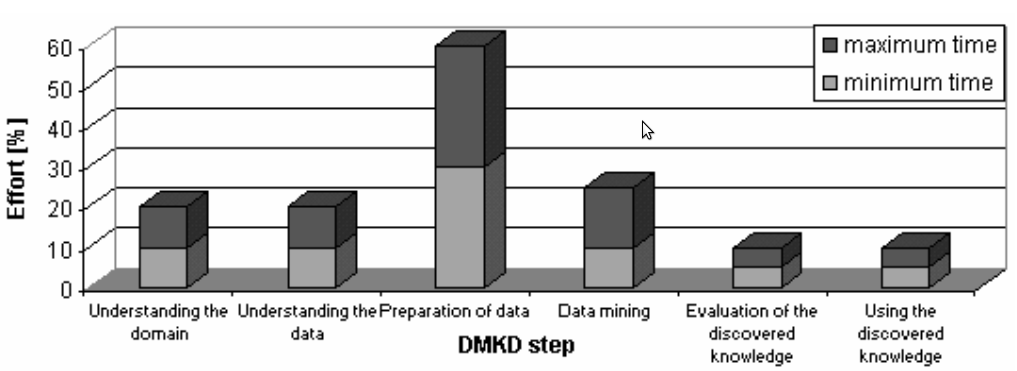
\includegraphics[width=0.7\textwidth]{imgs/preparation-time.png}
  \caption{Esforço relativo para cada passo do KDDM \citep{Cios2005}}
    \label{ap:fig:esforco}
\end{figure}

O \emph{framework} foi escrito em \emph{Python} e utiliza uma \emph{API} de
\emph{ORM} para esconder o serviço de banco de dados utilizado. Através dessa
modelagem o pesquisador tem simples acesso ao conjunto de membros da rede, ao
conjunto de suas interações (e propriedades) e a abrangência de cada. Nesse
quesito, precisamos separar o público-alvo esperado e o real (ver
\figref{ap:fig:grafo}), com isso, a atenção reflexiva é calculada em cima do
público-alvo esperado, enquanto que só o público-alvo direto cede atenção direta
para o autor. Com isso é possível que autores cedam mais do que recebem, à medida
que produzem para uma comunidade onde poucos ou nenhum de seus membros consomem
este conteúdo.

\begin{figure}[h!]
  \centering
    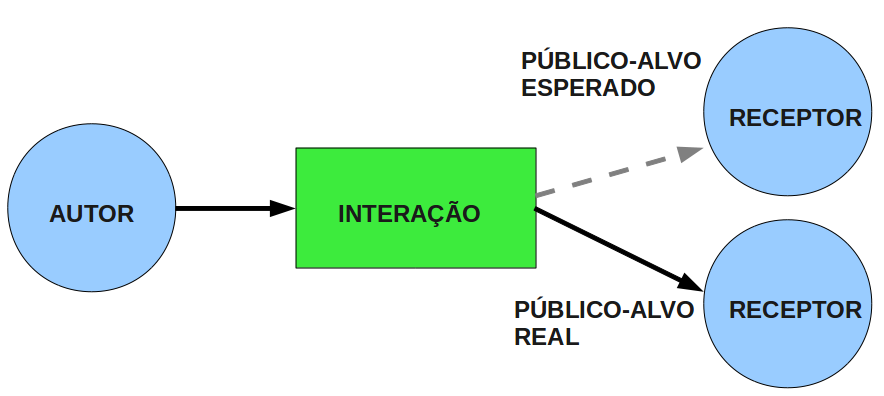
\includegraphics[width=0.7\textwidth]{imgs/naif-grafo.png}
  \caption{Exemplo de modelagem no \emph{framework}}
    \label{ap:fig:grafo}
\end{figure}

Implementamos o algoritmo de cálculo de atenção como apresentado na
\secref{sec:formalizacao}, e obtivemos o resultado separado para os dois grupos
de interações textuais: tópicos e resposta; histórias e comentários. O resultado
que encontramos é apresentado na \figref{ap:fig:cdf}, onde a distribuição da
carga de atenção parece seguir uma lei de potência. Essa característica é
interessante porque mimetiza a propriedade \emph{scale-free} das redes
sociais. 

As Figuras \ref{ap:fig:contatos}, \ref{ap:fig:topicos}, \ref{ap:fig:narrativas} e
\ref{ap:fig:completa} aprensentam visualizações das quatro redes concebidas: uma
não textual, que é a de contatos; três textuais, ou seja, utilizando nosso
algoritmo de atenção, sobre apenas tópicos e suas repostas, apenas histórias e
seus comentários e uma completa considerando tópicos e histórias. Na
\tabref{ap:tab:estatisticas} apresentamos algumas estatísticas sobre as quatro
redes, indicando grau médio de reciprocidade em todas as representações. Alto
grau de reciprocidade era esperado para as redes de atenção devido à atenção
residual, assim toda interação gera uma conexão da audiência para o autor e sua
recíproca do autor para a audiência, mesmo que em menor intensidade. O resultado
encontrado, principalmente na rede de tópicos, indica que apesar do autor da
mensagem visar obter a atenção de toda uma comunidade, poucos foram os que
efetivamente se prestaram a isso.

\begin{figure}[h!]
  \centering
    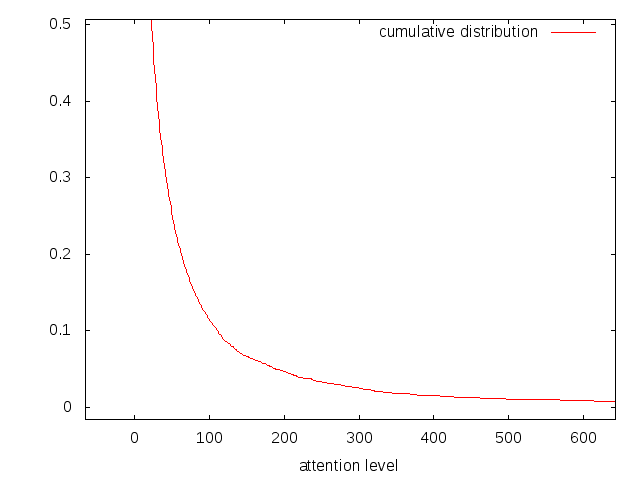
\includegraphics[width=0.7\textwidth]{imgs/cdf-final.png}
  \caption{Distribuição da Probabilidade Cumulativa da Atenção}
    \label{ap:fig:cdf}
\end{figure}

\begin{figure}[h!]
  \centering
    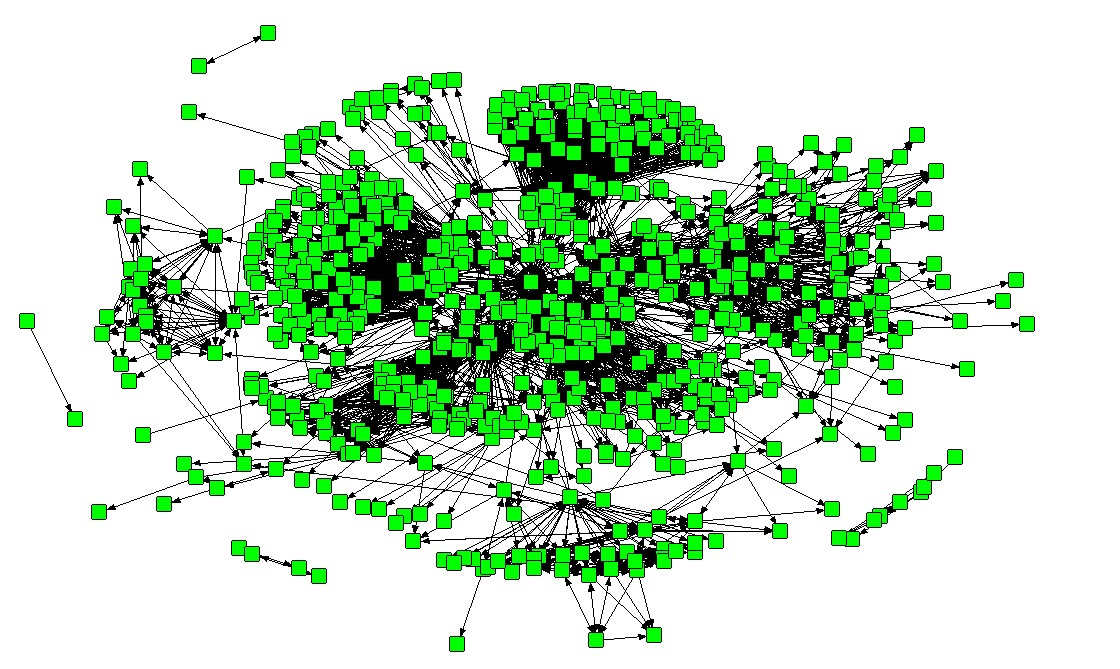
\includegraphics[width=0.7\textwidth]{imgs/contatos.jpg}
  \caption{Visualização da rede de contatos do a.m.i.g.o.s.}
    \label{ap:fig:contatos}
\end{figure}

\begin{figure}[h!]
  \centering
    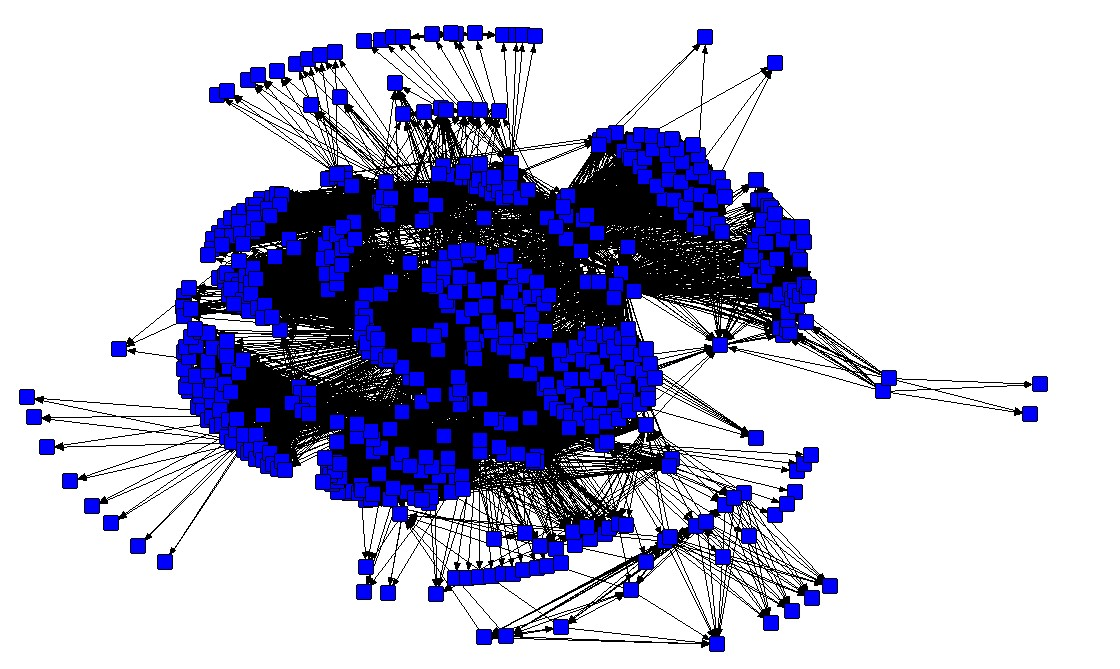
\includegraphics[width=0.7\textwidth]{imgs/topicos.jpg}
  \caption{Visualização da rede de tópicos do a.m.i.g.o.s.}
    \label{ap:fig:topicos}
\end{figure}

\begin{figure}[h!]
  \centering
    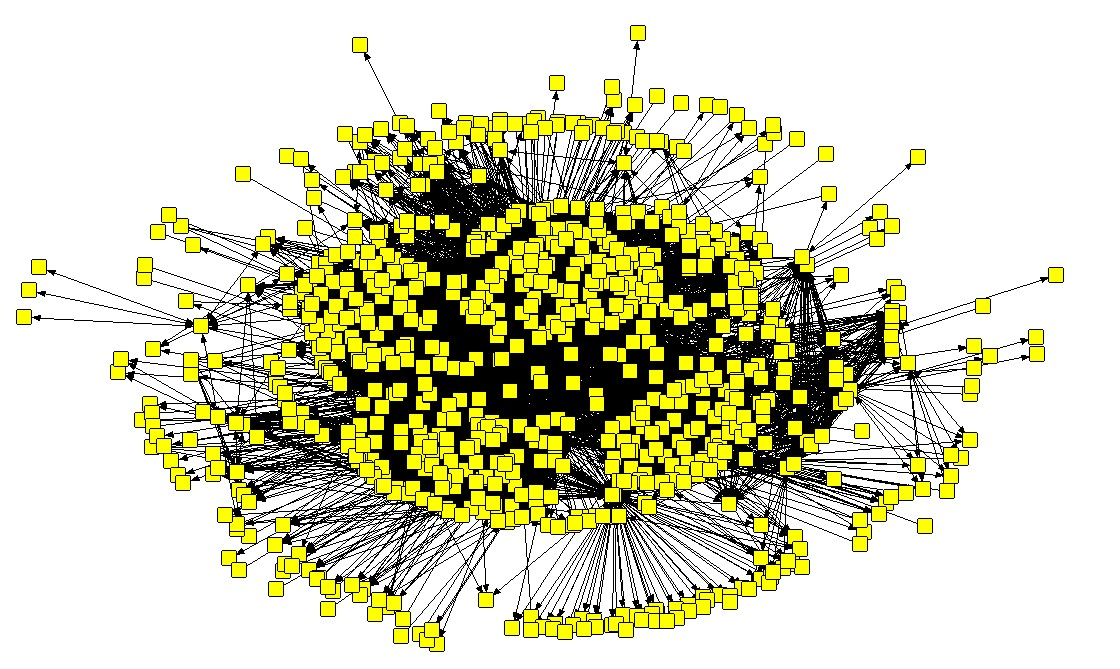
\includegraphics[width=0.7\textwidth]{imgs/narrativas.jpg}
  \caption{Visualização da rede de histórias do a.m.i.g.o.s.}
    \label{ap:fig:narrativas}
\end{figure}

\begin{figure}[h!]
  \centering
    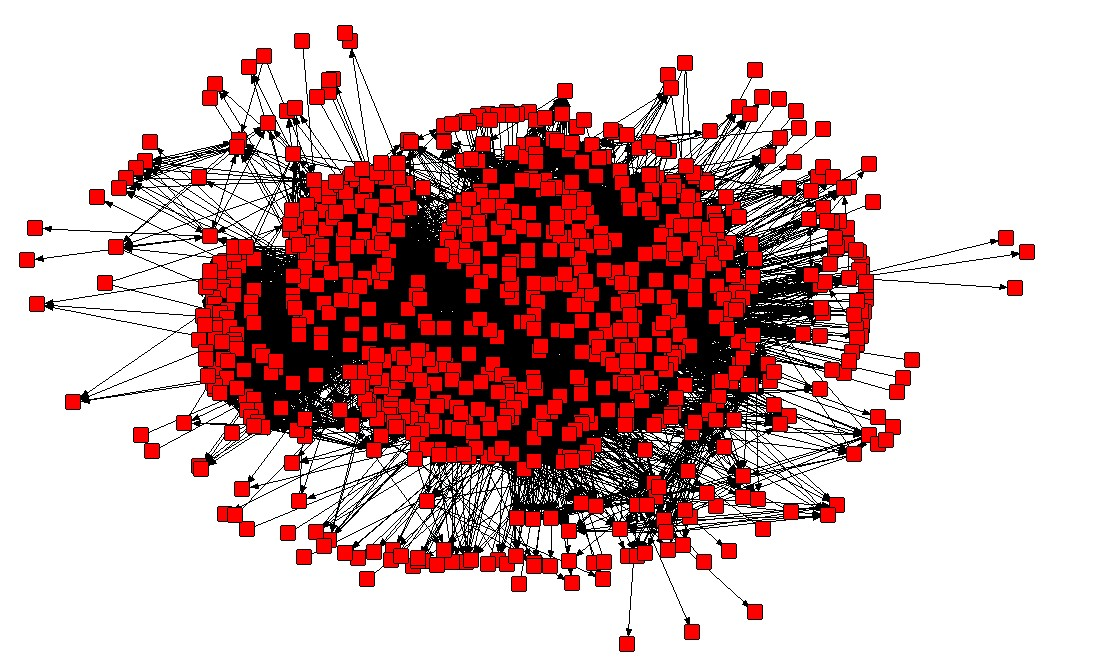
\includegraphics[width=0.7\textwidth]{imgs/completa.jpg}
  \caption{Visualização da rede de atenção completa do a.m.i.g.o.s.}
    \label{ap:fig:completa}
\end{figure}

\begin{table} [htbp]
	\large       % tamanho da fonte 
	\setlength{\arrayrulewidth}{2\arrayrulewidth}  % espessura da  linha
	\setlength{\belowcaptionskip}{10pt}  % espaço entre caption e tabela
	\caption{Tamanho e propriedades das redes} \centering   % tabela centralizada
	\begin{tabular}{| c | c | c | c | c |}
	\hline
	Rede & Tam. Componente & Densidade & Desv. Padrão & Reciprocidade \\ \hline
	Contatos & 680 & 0,01 & - & 0,55 \\
	Tópicos & 618 & 1,57 & 64,72 & 0,42\\
	Narrativa & 815 & 2,37 & 38,04 & 0,53\\
	Completa & 838 & 3,09 & 63,93 & 0,57\\ \hline
	\end{tabular}
	\label{ap:tab:estatisticas}
\end{table}

Antes de prosseguir com a análise da influência, podemos avaliar o quanto de
informação mútua existe nas redes mensuradas. Como foi mostrado na
\secref{sec:criterios}, redes com alto grau de sobreposição podem ser
descartadas uma em favor da outra para reduzir o conjunto a ser analisado na
próxima etapa. Na \tabref{ap:tab:qap} temos o resultado para as quatro redes
mensuradas. Se considerarmos separadamente tópicos e histórias, veremos que eles
tem pouca coisa em comum; mas a rede completa de atenção por sua vez é
fortemente correlacionada com ambas, sugerindo sua utilização no lugar das
primeiras. Também notamos uma leve para moderada correlação positiva entre a
rede de contatos e a de atenção, apesar de não estarem relacionadas diretamente.
Essa diferença entre as redes justificaria também uma forte diferença na análise
da influência?

\begin{table}[htbp]
	\large
	\setlength{\arrayrulewidth}{2\arrayrulewidth}
	\setlength{\belowcaptionskip}{10pt}
	\caption{\emph{QAP} aplicado as quatro redes (p. < 0,001)} \centering
	\begin{tabular}{|c | c  c  c  c |}
	\hline
	QAP corr & completa & contatos & histórias & tópicos \\ \hline
	completa & 1 & 0,22 & 0,67 & 0,82 \\
	contatos & 0,22 & 1 & 0,23 & 0,12 \\
	histórias & 0,67 & 0,23 & 1 & 0,13 \\
	tópicos	& 0,82 & 0,12 & 0,13 & 1 \\ \hline
	\end{tabular}
	\label{ap:tab:qap}
\end{table}


\section{Análise da influência}
\label{ap:sec:analise}

Após a mensuração das redes, apresentada na seção anterior, passamos à análise
de influência propriamente dita. Havíamos decidido usar o \emph{Flow
Betweenness} no passo 1 desse projeto, devido à natureza valorada da
representação, porém não nos foi possível alcançar nosso intento devido ao alto
custo computacional que se mostrou para essa métrica. Sendo assim, substituímos
pela métrica simples de \emph{Betweenness} que dicotomiza a rede pela média,
isto é, os laços cuja força seja maior ou igual que a média continuam (1) e os
abaixo são removidos (0). A métrica de \citeauthor{Bonacich1987} foi calculada
como planejada.

As Tabelas \ref{ap:tab:cent-contatos} e \ref{ap:tab:cent-completa} apresentam os
resultados para a métrica de \emph{Betweenness} nas rede de contatos e na de
atenção. No cabeçalho temos o índice de centralização de
\citeauthor{Freeman1979} que indica o quão próximo a rede está de um gráfico do
tipo estrela. É interessante notar que a rede de atenção formada apenas com os
tópicos e suas resposta apresentou o maior grau de centralização: 37,18\%;
enquanto que as histórias apresentaram: 24,20\%. Destacamos em negrito os
membros que se repetiram nas quatro representações: contatos, tópicos, histórias
e completa. É interessante notar que apesar não haver nenhuma relação direta
entre a rede completa e a de contatos, aquela manteve quase que inalterada a
ordenação do grupo que intersecta ambas.

\begin{table}[htbp]
	\large       % tamanho da fonte 
	\setlength{\arrayrulewidth}{2\arrayrulewidth}  % espessura da  linha
	\setlength{\belowcaptionskip}{10pt}  % espaço entre caption e tabela
	\caption{Os 9 membros mais bem posicionados na rede de Contatos} \centering   
	\begin{tabular}{| c | c |}
	\hline
	Contatos & Centralização=30,81\% \\ \hline\hline
	Membro & \emph{Betweenness} \\ \hline
	\textbf{3} & \textbf{31,06} \\
	\textbf{8} & \textbf{13,48} \\
	135 & 11,44 \\
	\textbf{2} & \textbf{8,68} \\
	\textbf{200} & \textbf{5,14} \\
	201 & 4,84 \\
	\textbf{796} & \textbf{4,82} \\
	601 & 4,57 \\
	665 & 4,55 \\ \hline
	\end{tabular}
	\label{ap:tab:cent-contatos}
\end{table}

\begin{table}[htbp]
	\large       % tamanho da fonte 
	\setlength{\arrayrulewidth}{2\arrayrulewidth}  % espessura da  linha
	\setlength{\belowcaptionskip}{10pt}  % espaço entre caption e tabela
	\caption{Os 9 membros mais bem posicionados na rede de Atenção} \centering   
	\begin{tabular}{| c | c |}
	\hline
	Completa & Centralização=23,07\% \\ \hline\hline
	Membro & \emph{Betweenness} \\ \hline
	\textbf{3} & \textbf{23,18} \\
	\textbf{2} & \textbf{12,53} \\
	\textbf{8} & \textbf{8,99} \\
	\textbf{200} & \textbf{3,65} \\
	\textbf{796} & \textbf{3,37} \\
	6 & 1,79 \\
	665 & 1,7 \\
	397 & 1,61 \\
	201 & 1,5 \\\hline
	\end{tabular}
	\label{ap:tab:cent-completa}
\end{table}

Quando analisamos a correlação entre os resultados de centralidade das quatro
redes mensuradas, apresentada na \tabref{ap:tab:cent-corr}, podemos perceber o
impacto da decisão em usar a métrica de \emph{Betweenness} no lugar da original.
A dicotomização da rede quase que totalmente mimetiza o padrão de posicionamento
encontrado na rede de contatos; i.e., removido o peso dos laços, parece-nos que
os atores fazem as mesmas escolhas em termos de quem interagir e de quem
adicionar aos seus contatos. Entretando, o índice de \citeauthor{Bonacich1987}
leva em consideração este peso para a rede de atenção, logo seus resultados
devem se diferenciar bastante da rede não-textual.

\begin{table}[htbp]
	\large       % tamanho da fonte 
	\setlength{\arrayrulewidth}{2\arrayrulewidth}  % espessura da  linha
	\setlength{\belowcaptionskip}{10pt}  % espaço entre caption e tabela
	\caption{Correlação do índice de centralidade} \centering   
	\begin{tabular}{| c | c c c c|}
	\hline
	\emph{Betweenness} & completa & contatos & histórias & tópicos \\ \hline
	completa & 1 & 0,89 & 0,96 & 0,94 \\
	contatos & 0,89 & 1 & 0,91 & 0,87 \\
	histórias & 0,96 & 0,91 & 1 & 0,93 \\
	tópicos & 0,94 & 0,87 & 0,93 & 1 \\\hline
	\end{tabular}
	\label{ap:tab:cent-corr}
\end{table}

Para o índice de prestígio, temos grande disparidade nos resultados apresentados
pelas redes textuais e não-textuais, como era de se esperar. As Tabelas
\ref{ap:tab:prest-contato} e \ref{ap:tab:prest-completa} nos traz os melhores
colocados no índice de \citeauthor{Bonacich1987} para as redes de contatos e de
atenção respectivamente. Da mesma forma como nas de centralidade, os membros que
se repetiram nas melhores colocações em todas as quatro redes foram marcados em
negrito; neste caso, houve apenas um. Esse resultado nos diz que apesar de
estruturalmente a rede de atenção ser similar a de contatos, quando levamos em
consideração a intensidade dessas interações, a distribuição desigual da atenção
nos revela os influenciadores realmente ativos.

\begin{table}[htbp]
	\large       % tamanho da fonte 
	\setlength{\arrayrulewidth}{2\arrayrulewidth}  % espessura da  linha
	\setlength{\belowcaptionskip}{10pt}  % espaço entre caption e tabela
	\caption{Os 9 membros mais prestigiados na rede de Contatos} \centering   
	\begin{tabular}{| c | c |}
	\hline
	\citeauthor{Bonacich1987} & Contatos\\ \hline\hline
	Membro & \emph{Power} \\ \hline
	8 & 240,311 \\
	\textbf{3} & \textbf{189,279} \\
	397 & 128,291 \\
	385 & 120,024 \\
	419 & 119,683 \\
 	481 & 109,363 \\
 	422 & 108,501 \\
 	436 & 106,941 \\ 
 	452 & 106,314 \\\hline
	\end{tabular}
	\label{ap:tab:prest-contato}
\end{table}

\begin{table}[htbp]
	\large       % tamanho da fonte 
	\setlength{\arrayrulewidth}{2\arrayrulewidth}  % espessura da  linha
	\setlength{\belowcaptionskip}{10pt}  % espaço entre caption e tabela
	\caption{Os 9 membros mais prestigiados na rede de Atenção} \centering   
	\begin{tabular}{| c | c |}
	\hline
	\citeauthor{Bonacich1987} & Atenção\\ \hline\hline
	Membro & \emph{Power} \\ \hline
	2 & 649,7 \\
	665 & 304,450 \\
	681 & 264,112 \\
	711 & 205,687 \\
	668 & 132,357 \\
	\textbf{3} & \textbf{108,871} \\
	201 & 104,042 \\
	781 & 79,441 \\
	826 & 76,397 \\\hline
	\end{tabular}
	\label{ap:tab:prest-completa}
\end{table}

Como era de se esperar, não poderíamos ter muita compatibilidade entre o
resultado de contatos e o de atenção. A \tabref{ap:tab:prest-corr} nos confirma
isso, mas também nos indica que a quase totalidade (98\%) do prestígio advém
das interações nos fóruns (tópicos e respostas). Certamente também
encontraríamos essa diferença na centralidade se não tivessemos dicotomizado os
dados.

\begin{table}[htbp]
	\large       % tamanho da fonte 
	\setlength{\arrayrulewidth}{2\arrayrulewidth}  % espessura da  linha
	\setlength{\belowcaptionskip}{10pt}  % espaço entre caption e tabela
	\caption{Correlação do índice de prestígio} \centering   
	\begin{tabular}{| c | c c c c|}
	\hline
	\emph{Betweenness} & completa & contatos & histórias & tópicos \\ \hline
	completa & 1 & 0,07 & 0,1 & 0,98 \\
	contatos & 0,07 & 1 & 0,28 & 0,06 \\
	histórias & 0,1 & 0,28 & 1 & 0,06 \\
	tópicos & 0,98 & 0,06 & 0,06 & 1 \\\hline
	\end{tabular}
	\label{ap:tab:prest-corr}
\end{table}

Finalmente, avaliamos a utilidade das métricas calculadas tendo por base o que
foi apresentado na \secref{sec:rel_proe}. Sendo assim, caso a rede mensurada
não tenha propriedades estruturais de uma comunidade de prática, então a métrica
radial que escolhemos, o poder de \citeauthor{Bonacich1987}, terá pouca
utilidade prática já que os \emph{hubs} estarão isolados em seus
\emph{clusters}. A \tabref{ap:tab:comu_prat} nos mostra que esse não é o caso,
encontramos um alto grau de coesão e padrão núcleo/periferia nas redes
mensuradas. Sendo a rede de tópicos a que mais se destacou com esse padrão,
talvez por representar o dia a dia dos colaboradores em suas trocas de
mensagens.

\begin{table}[htbp]
	\large       % tamanho da fonte 
	\setlength{\arrayrulewidth}{2\arrayrulewidth}  % espessura da  linha
	\setlength{\belowcaptionskip}{10pt}  % espaço entre caption e tabela
	\caption{Indícios de comunidades de prática} \centering   
	\begin{tabular}{| c | c | c | c | c |}
	\hline
	 & completa & contatos & histórias & tópicos \\ \hline
	Coeficiente Clusterização & 0,68 & 0,55 & 0,66 & 0,74 \\
	Coef. Cluster. Ponderado & 0,5 & 0,26 & 0,5 & 0,4 \\
	Distância média & 2,84 & 3,82 & 2,64 & 1,72 \\
	Adequação Núcleo/Perif. & 0,52 & 0,02 & 0,38 & 0,62 \\\hline
	\end{tabular}
	\label{ap:tab:comu_prat}
\end{table}

Para ilustrar a aplicação desse novo conhecimento adquirido, vamos utilizar uma
quinta e ultima mensuração do a.m.i.g.o.s.: a rede de recomendação. A rede de
atenção se comporta de certa forma às avessas, se um laço vai de $a$ para $b$ é
por que houve uma interação de $b$ para $a$. Então temos que prestígio, na rede
atenção, é sinônimo de atividade; Usuários ativos que publicam muito conteúdo
recebem muita atenção e por isso possuem alto prestígio. Para testar essa
afirmação, mensuramos uma rede binária direcionada ingênua a partir das
recomendações encontradas no sistema. Nessa representação, se $X_{ab}=1$ então
$a$ enviou uma recomendação de algo (comunidade, tópico ou história) para $b$.
Só pra constar, recomendações são interações de conteúdo não-textual e de
abrangência individual básica (i.e., de membro a membro), no geral, sua
intenção é informativa ou conectiva.

\begin{figure}[h!]
  \centering
    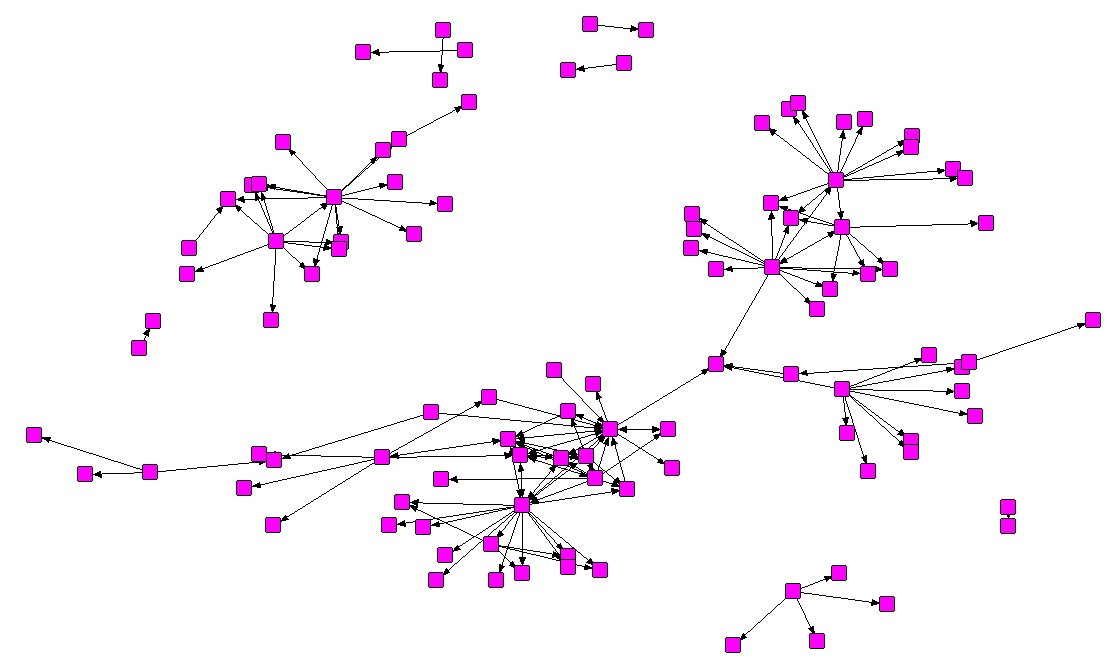
\includegraphics[width=0.7\textwidth]{imgs/recmd.jpg}
  \caption{Visualização da rede de recomendação do a.m.i.g.o.s.}
    \label{ap:fig:recmd}
\end{figure}

Para o caso de uma rede como a da \figref{ap:fig:recmd}, temos que os atores
mais centrais são também os mais ativos, por que recomendam algo aos outros.
Neste caso em particular, como foram poucas recomendações registradas no sistema
até o momento em que nos foi fornecido o acesso, calculamos apenas 10 atores com
alguma centralidade. Se o prestígio em nossa rede de atenção mede realmente a
intensidade que um membro atua no ambiente, então é de se esperar que
encontremos uma forte interseção entre esses dois conjuntos (prestígio na rede
de atenção e centralidade na rede de recomendação).

É exatamente o que encontramos, os 5 membros mais centrais nas recomendações já
aparecem na lista dos 10 mais em prestígio. Encontramos até o 9 na  lista dos 100
mais e o último colocado nas recomendações ocupa o 210\textordmasculine~lugar
na de prestígio. Quanto a ordenação, encontramos uma correlação espantosa entre os
dois atributos: 0,929. O que indica que com muita pouca variação, quem tem mais
prestígio também recomendou mais.

E no caso da centralidade para redes de atenção, o que representa? No nosso
caso, pouco devido à dicotomização da rede que mascarou a diferença entre
autores e receptores. Entretanto, considerando o uso da \emph{Flow Betweenness}
original, o esperado é que os atores centrais fossem aqueles com muitas ligações
fortes entre vários atores, isto quer dizer que são membros receptores que se
posicionam na rede consumindo informação de fontes variadas. Esses receptores
atuam então como \emph{brokers} repassando as informações que acham válidas. 

Em uma utilização do resultado desse exercício para o marketing ou a simples
divulgação de informação, deveriamos visar primeiro os de alto prestígio, esses
serão aqueles onde a cascata começará, mas também não devemos esquecer dos de
alta centralidade. Se no propagar da cascata a novidade encontrar um
\emph{broker} já inclinado a aceitar, a probabilidade vai ser muito maior da
onda se espalhar em novos ambientes.

\section{Resultados encontrados}
\label{ap:sec:resultados}

Em primeiro lugar, o resultado positivo encontrado nos dados para as hipóteses
levantadas no começo do processo, sugere que o método de mineração de dados
serviu seu propósito de orientar a pesquisa com segurança. A tipologia de
interações e o \emph{framework} conceitual que descrevemos no decorrer desse
trabalho, aplicaram-se adequadamente ao estudo de caso. Não obstante disso
deduza-se necessariamente sua aplicabilidade a outros tipos de casos,
acreditamos que ele foi definido geral o suficiente para tal.

Inesperadamente, talvez por necessidade, também iniciamos a construção de uma
ferramenta simples para o auxílio na preparação dos dados. Em uma busca rápida ao
site da \emph{Internacional Network for Social Network Analysis}
\citep{INSNA2010} encontramos de um total de 29 \emph{softwares} catalogados para
o uso em SNA, desses observamos: 11 são para visualização da rede, 5 são pacotes
estatísticos e matemáticos, 2 são de transformação de dados (XML e áudio), 8 são
voltados para algoritmos de SNA propriamente, como o UCINET \citep{Borgatti2010}
que foi usado para calcular as métricas nesse estudo de caso) e 3 envolvem a
extração dos dados propriamente dita. Desses últimos, o que mais se aproxima da
ferramenta desenvolvida nesse projeto é o UrlNet \citep{Hunscher2010} que
facilita a criação de \emph{crawlers} para a \emph{web}; curiosamente também
desenvolvido na linguagem Python. Mesmo assim, acreditamos que há espaço para a
nossa ferramenta, pois é de propósito geral e permite reunir o resultados dos
\emph{crawlers} em modelos: membros x interação.

 



\end{document}